\lhead{\emph{Multiresolution Sinusoidal Neural Networks}}
\chapter{Multiresolution Sinusoidal Neural Networks}
\label{chap:mr_snn}

In this chapter, we present a novel family of neural network architectures designed to efficiently encode signals at multiple scales. Our objective is to construct a continuous, compact, and high-fidelity representation of scalar and vector fields, making it applicable to a variety of media such as audio, images, shapes, and complex spatiotemporal data. These media objects, interpreted as signals, can be given explicitly as attributes of space-time coordinates or implicitly as level sets of functions.

This chapter builds upon our exploration of sinusoidal neural networks, where we analyzed how frequency capacity and initialization schemes influence the network's ability to represent diverse signal frequencies. Drawing on these insights, we propose a multiresolution neural network (MR-Net) architecture that combines classical multi-scale signal processing techniques with modern deep learning methodologies to address the limitations of existing coordinate-based models.

The MR-Net framework introduces a unified architecture capable of encoding signals in a multiscale manner, supporting flexible training regimes and progressive refinement. It includes three primary subclasses, each designed for distinct frequency control scenarios: \emph{S-Net}, \emph{L-Net}, and \emph{M-Net}. These subclasses offer different trade-offs between frequency resolution and control, and computational efficiency, providing a versatile toolkit for representing complex signals across a range of applications.

To implement the multiresolution approach, we draw inspiration from classical signal processing techniques such as Gaussian and Laplacian pyramids. In MR-Net, levels of detail are determined by spectral projections, and training proceeds in a progressive manner, refining the representation incrementally. The preliminary versions of MR-Net were first presented in \cite{paz2022,paz2023mr}. In the following sections, we describe the theoretical foundations, design principles, and architectural details of MR-Net, providing a comprehensive overview of the framework and its potential applications.

% Key features of the MR-Net framework include:

% \begin{itemize}
%     \item \textbf{Flexible Data Handling}: MR-Net can be trained with various types of data, including regularly sampled grids, hierarchical multiresolution structures such as pyramids, or through stochastic and stratified sampling.
%     \item \textbf{Adaptive Level of Detail}: The network can adapt its representation to match the input data's resolution. For multiresolution training, levels of detail are determined by spectral projections, while for single-resolution inputs, they are governed by the network's capacity and initialization control.
%     \item \textbf{Progressive Training Paradigms}: Training proceeds in a progressive manner, refining the representation incrementally. This approach ensures efficient learning across a range of scales and improves convergence for high-frequency details.
%     \item \textbf{Continuous Multiscale Representation}: The MR-Net architecture encodes signals in a continuous manner, both in spatial and scale dimensions, enabling seamless reconstruction at arbitrary resolutions.
% \end{itemize}

% For the multiresolution approach, we leverage classical structures of image and signal processing, such as Gaussian and Laplacian Pyramids. We use these ideas to develop a framework to train a multi-stage neural network using multiresolution structures in an efficient way. \red{Finally, we demonstrate that our model can achieve a comparable reconstruction quality to a simple SIREN model with the same number of parameters, while encoding multiple levels of detail. Esta frase deve ser movida para o capítulo seguinte, de aplicações em imagens. A conclusão desta parte será finalizada quando este capítulo estiver completo.}

% \red{We have established that we can bound the frequencies learned by a sinusoidal neural network by adjusting the interval of frequencies sampled for initialization of its first layer, and also by adjusting the network capacity. That is, if the value of $\omega_0$ is too low, the network will learn the lower frequencies of the signal, fitting their intensities in the Fourier spectrum, but won't learn the higher frequencies, even if it has enough computational units to to do. On the other hand, if the capacity given by the computational units is too small, the result will also resemble a filtered version of the target signal. TALVEZ MOVER PARA O CHAPTER 4 - MR-TRAINING}

\section{Related Works}

\sloppy Multiresolution analysis has its roots in the seminal work of~\citep{mallat1989theory} and \citep{daubechies92}, who formalized the wavelet transform as a powerful tool for analyzing signals at different scales. Their contributions provided the framework for decomposing signals into distinct frequency bands while preserving spatial or temporal information, which is essential for many signal processing applications.

Integrating multiresolution concepts with neural network architectures has led to several innovative developments. One such approach is the scattering networks proposed by \citet{bruna2013}, which apply cascaded wavelet transforms followed by nonlinear operators to produce stable, translation-invariant signal representations. For image-related tasks, architectures such as those by \citet{sppHe2015} and \citet{YuKoltun2016} employ Convolutional Neural Networks (CNNs) to process inputs at multiple scales simultaneously. However, these models are primarily designed to extract features from large datasets for applications like image classification, rather than to represent signals in a multiresolution format.

\citet{zhangWavelet92} introduced Wavelet Neural Networks (WNNs), which leverage wavelet functions as activation units, replacing traditional perceptrons with \textit{wavelons} to perform adaptive wavelet transforms on input signals. While WNNs offer a novel alternative to perceptron-based neural networks, some inherent limitations might have prevented further development on this approach. First, unlike deep neural networks that learn hierarchical features, WNNs architectures are shallow and, thus, require a significantly larger number of parameters to achieve high-fidelity signal representation. Furthermore, WNNs can be challenging to optimize, with their performance heavily influenced by the initial choice of wavelet functions and corresponding parameters.

In the domain of coordinate-based neural networks, \citet{bacon2021} introduced the Band-Limited Coordinate Network (BACON), which is built on the Multiplicative Filter Network architecture \citep{fathony2020multiplicative}. BACON generates intermediate outputs with predefined spectral bandwidth, achieving multiresolution representations of underlying signals. While its structure avoids the composition of sines present in deep sinusoidal MLPs, allowing BACON to be expressed as a linear combinations of sines, it creates multiresolution representations by truncating the frequency spectra of the signals at a specific value. This method introduces ringing artifacts at certain levels of detail, as evident in the Fourier transforms of images reconstructed using BACON (see Chapter \ref{ch:imaging}).

% The ability to control frequency bands in representation is closely tied to the capability of adaptively reconstructing signals at multiple levels of detail. \citet{mueller2022instant} developed a multiresolution neural network architecture based on hash encoding, while \citet{martel2021acorn} designed an adaptive coordinate network for neural signals.

% Frequency band control is crucial for adaptively reconstructing signals across multiple levels of detail. Recent works have explored this idea: \citet{mueller2022instant} presented a multiresolution neural network based on hash encoding, and \citet{martel2021acorn} proposed ACORN, an adaptive coordinate network for representing neural signals. Both works offer adaptive or dynamic data structures combined with neural networks for refining representations, focusing on efficient memory usage or grid refinement, but lack interpretability of frequency control and are not suitable for continuous multiresolution.

\citet{martel2021acorn} proposed ACORN, an adaptive coordinate network for representing neural signals, while \citet{mueller2022instant} introduced a multiresolution neural network utilizing hash encoding. Both approaches leverage adaptive or dynamic data structures combined with neural networks to refine representations, with a focus on efficient memory usage and grid refinement. However, these methods lack explicit frequency control and are not inherently designed for continuous multiresolution, which limits their interpretability in controlling signal frequencies across different levels of detail.

In this context, we introduce \textit{Multiresolution Sinusoidal Neural Networks} (MR-Net) \citep{paz2022,paz2023mr} based on classical signal multiresolution representations. Our results in imaging applications, discussed in Chapter \ref{ch:imaging}, demonstrate that MR-Net outperforms the previous state-of-the-art technique, BACON, while utilizing a smaller number of parameters.


% # Weaknesses of Wavelet Neural Networks

% ## 1. Training Complexity

% - WNNs often require optimization of wavelet parameters (scaling and translation) along with the usual network weights.
% - This increases the number of parameters to be learned, potentially leading to longer training times and increased risk of overfitting.
% - The optimization landscape can be more complex, with many local minima, making it challenging to find optimal solutions.

% ## 2. Limited Representational Capacity

% - While effective for certain types of signals, WNNs may struggle with very complex or high-dimensional data.
% - The fixed wavelet basis might not be optimal for all types of signals or tasks.
% - Compared to modern deep learning architectures, WNNs often have lower representational capacity, limiting their performance on complex tasks.

% ## 3. Lack of Hierarchical Feature Learning

% - Unlike deep neural networks that learn hierarchical features, WNNs typically have a shallow architecture.
% - This can limit their ability to capture complex, multi-level abstractions in the data.
% - The absence of multiple layers of nonlinear transformations can restrict the network's ability to learn intricate patterns.

% ## 4. Sensitivity to Initial Conditions

% - The performance of WNNs can be highly dependent on the initial choice of wavelet functions and their parameters.
% - Poor initialization can lead to suboptimal results or slow convergence during training.

% ## 5. Limited Adaptability

% - Once trained, the wavelet basis in WNNs is fixed, which can limit their adaptability to new, unseen data.
% - This contrasts with some modern architectures that can adapt their feature extraction process more flexibly.

% Título Alternativo "Multiresolution Signal Decomposition"
\section{Multiscale Representation and Learning}
\label{s-motivation}

Let $\gt{f}:\mathcal{D}\to \mathcal{C}$ be a \textit{ground-truth signal}, where $\mathcal{D}$ and $\mathcal{C}$ are finite-dimensional vector spaces representing the signal's domain and codomain, respectively. For example, to represent an image, $\mathcal{D}$ could be set to $\R^2$ to define the spatial domain, while $\mathcal{C}=\R^3$ corresponds to the RGB color space. Throughout this text, we use cursive fonts to denote ground-truth signals and a standard font for their corresponding neural network approximations.

To represent the signal $\gt{f}$ at multiple scales, we decompose it into a sum of $N$ stages: $\gt{f}=\gt{g}_0+\dots+\gt{g}_{N-1}$, where $\gt{g}_0$ captures the coarsest approximation of the signal and $\gt{g}_i$, for $i>0$, progressively introduces higher-frequency components. This multiresolution decomposition allows us to define the \textit{level of detail} at stage $i$ in two equivalent forms:

\begin{equation}
\gt{f}_i = \gt{g}_0 + \cdots + \gt{g}_i \quad \text{or} \quad \gt{f}_i = \gt{f} - \sum_{j=i+1}^{N-1} \gt{g}_j.
\end{equation}

Each stage $\gt{g}_i$ is computed as:
\begin{equation}
\gt{g}_i = \gt{f}_{i+1} - K * \gt{f}_{i+1}, \quad \text{where } \gt{f}_{N-1} = \gt{f}.
\end{equation}

In this formulation, each stage $\gt{g}_i$ represents the difference between the $(i+1)$-th level of the signal and its smoothed version, obtained by convolving it with a low-pass filter $K$. For instance, $K$ may be a \textit{Gaussian kernel} of the form $G(x,t)=\frac{1}{2\pi t}\exp{\left(-\frac{\|x\|^2}{2t}\right)}$, where $t$ is a scale parameter that controls the degree of smoothing. This way, the sequences $\{\gt{f}_i\}$ and $\{\gt{g}_i\}$ correspond to the \textit{Gaussian} and \textit{Laplacian} pyramids, respectively, which are well-established tools in multiresolution analysis of digital images \citep{lindeberg1994scale, velho2009image, rosenfeld2013multiresolution}.

Given this multiscale decomposition, our goal is to represent the signal $\gt{f}$ using a family of sinusoidal neural networks. Motivated by the hierarchical structure of $\gt{f}=\gt{g}_0+\dots+\gt{g}_{N-1}$, we propose using an aggregation of $N$ sinusoidal MLPs, denoted by $g_i:\mathcal{D}\to \mathcal{C}$, to approximate each stage $\gt{g}_i$. By training each $g_i$ to match its corresponding stage $\gt{g}_i$, we gain precise control over the frequency spectrum learned by each network. This design leverages the spectral bias of sinusoidal networks, as discussed in Chapter \ref{chap:sinusoidal}, allowing the network to naturally prioritize lower frequencies and gradually introduce higher-frequency details.

Each network stage $g_i$ is initialized with a specific and crescent range of frequencies, ensuring that the resulting approximation accurately matches the desired stage $\gt{g}_i$. This structured frequency learning approach enables the decomposition and reconstruction of complex signals in a manner that is both progressive and controlled.

\section{MR-Net Architecture}

The MR-Net architecture is a family of continuous multiresolution networks designed to approximate a complex signal by progressively adding details at multiple levels of resolution. The architecture is defined as a function \( f:\mathcal{D} \times [0,N] \to \mathcal{C} \), where \(\mathcal{D}\) and \(\mathcal{C}\) represent the domain and codomain of the signal, respectively. Formally, the MR-Net is expressed as follows:

\begin{align}\label{e-mrnet}
f(x,t) = c_0(t) g_0(x) + \cdots + c_{N-1}(t) g_{N-1}(x),
\end{align}

where each function \( g_i : \mathcal{D} \to \mathcal{C} \) is a \textbf{Multiresolution (MR) Module} —a building block of the MR-Net that is defined in detail in Sec~\ref{s-mr-module}. The MR-Net is composed of \( N \) such MR Modules, each corresponding to a different stage in the multiresolution hierarchy of \( f \). 

The contributions of each MR-Module \( g_i \) are controlled by a set of blending functions \( c_i(t) \), defined as:

\begin{align}\label{e-control}
c_i(t) = \max \Big\{ 0, \min \big\{ 1, t - i \big\} \Big\}.
\end{align}

Intuitively, this function ensures that:

\begin{itemize}
    \item When \( t < i \), \( c_i(t) = 0 \).
    \item When \( i \leq t \leq i+1 \), \( c_i(t) = t - i \).
    \item When \( t > i + 1 \), \( c_i(t) = 1 \).
\end{itemize}

Therefore, if \( t = k + \delta \) (with \( k \in \mathbb{N} \) and \( 0 \leq \delta \leq 1 \)), we can express \( f(x, t) \) as the linear combination:

\begin{align}
f(x, t) = g_0(x) + \cdots + g_k(x) + \delta \, g_{k+1}(x).
\end{align}

Each stage function \( f_t := f(\cdot, t) : \mathcal{D} \to \mathcal{C} \) defines a \textit{level of detail} parameterized by \( t \). The resulting MR-Net $f$ learns the decomposition of the ground-truth signal $\gt{f}$ as a projection into the coarse scale space and a sequence of finer detail spaces. For instance, the initial stage $f_1=g_0$ provides the least detailed approximation~of~$f_N$. As \( t \) evolves from 0 to \( N \), these stages progressively refine the representation of the signal, with \( f_N = g_0 + \cdots + g_{N-1} \) representing the full-resolution approximation.

To train this architecture, we fit \( f \) to the ground-truth signal \( \gt{f} = \gt{g}_0 + \cdots + \gt{g}_{N-1} \) by initializing and training each stage \( g_i \) to approximate the corresponding stage of the ground-truth decomposition. In Section \ref{s:training}, we provide more details on training.

This structure aligns with the concept of Multiresolution Analysis~\citep{mallat1989theory}, where a function is decomposed into a sequence of approximations and detail spaces, each stage refining the approximation of the original signal. The MR-Net enables a continuous traversal through these stages using the scale parameter \(t\), allowing seamless navigation across multiple resolutions. Fig.~\ref{f:mrnet-arch} shows the general architecture of an MR-Net having \(N\) stages.

\begin{figure}[!h]
\centering
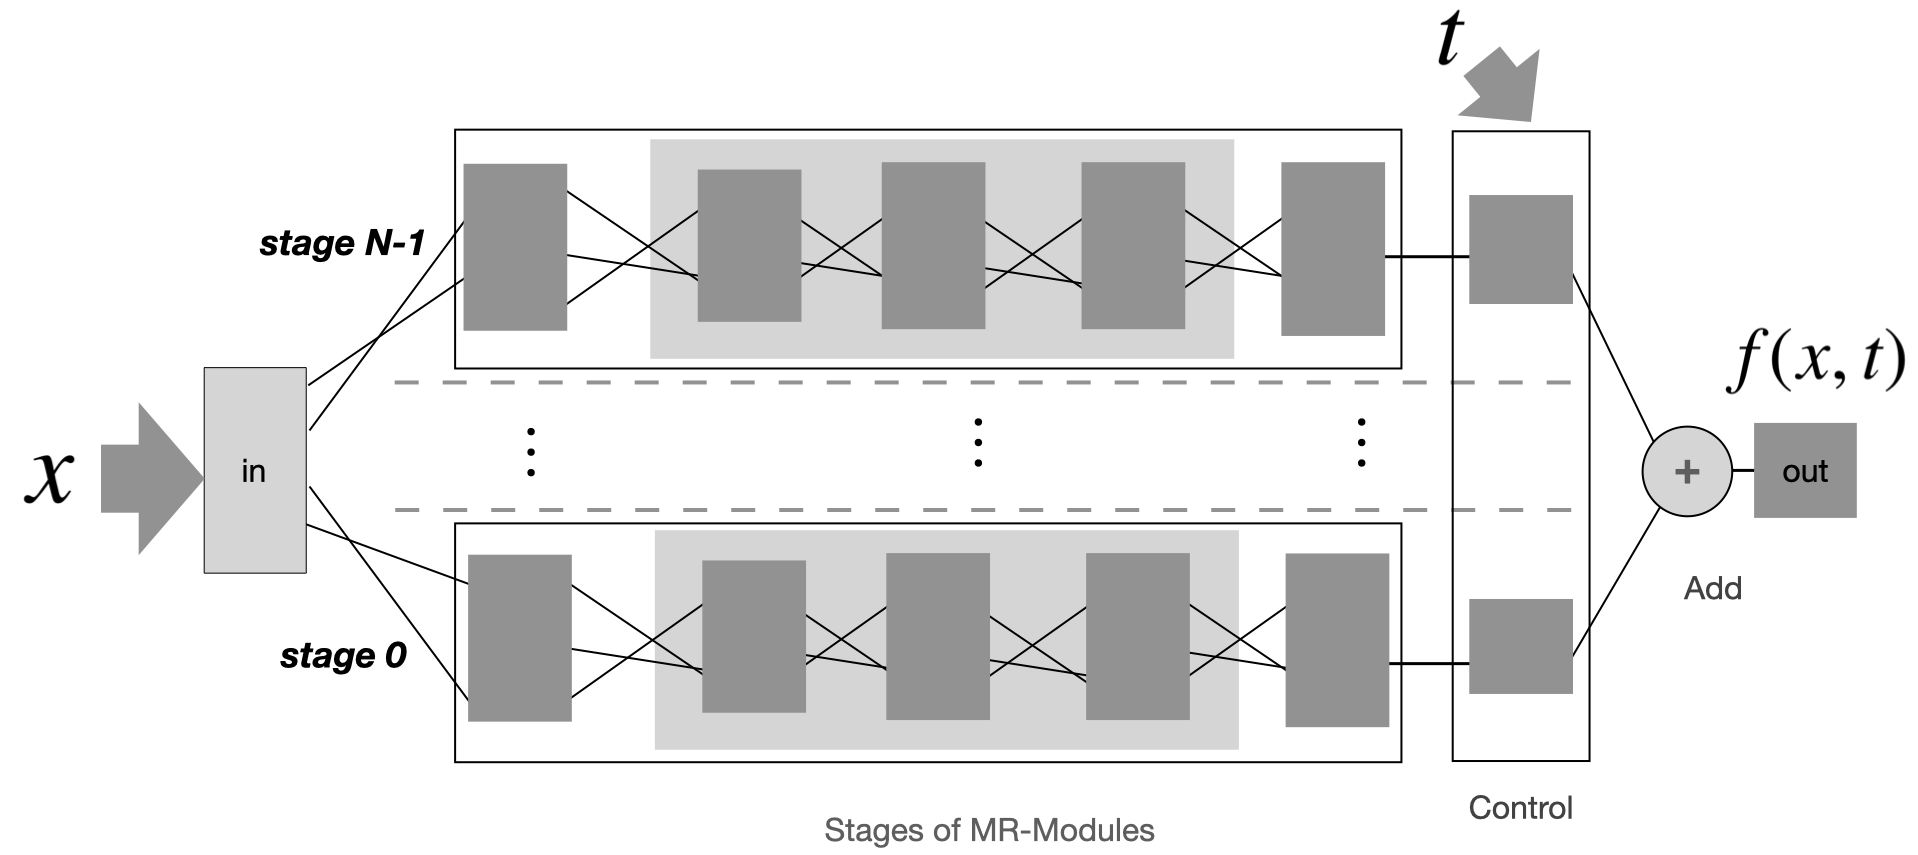
\includegraphics[width=0.9\linewidth]{img/ch4/mr-net-stages-v2.png}
\caption{Anatomy of the MR-Net Family.}
\label{f:mrnet-arch}
\end{figure}


\subsection{MR-Module}
\label{s-mr-module}

Each stage \( g_i \) in the MR-Net is a \textit{Multiresolution (MR) Module}, defined as a sinusoidal MLP with induced frequency bands. A MR-Module is constructed as a function \( g_i = L_i \circ H_i \circ S_i \), illustrated in the Figure \ref{f:mr-module}, where:

\begin{itemize}
    \item \( S_i \): The first sinusoidal layer that projects the input \( x \in \mathcal{D} \) into a list of sines, generating \( S_i(x) \).
    \item \( H_i \): A sequence of hidden layers (optional), composed of \( k \) intermediate transformations of the sines. The output $H_i\circ S_i(x)$ is a dictionary of sine combinations.
    \item \( L_i \): The final linear layer that combines these transformed sine functions, serving as the atoms of a representation dictionary.
\end{itemize}


\begin{figure}[!h]
    \centering
    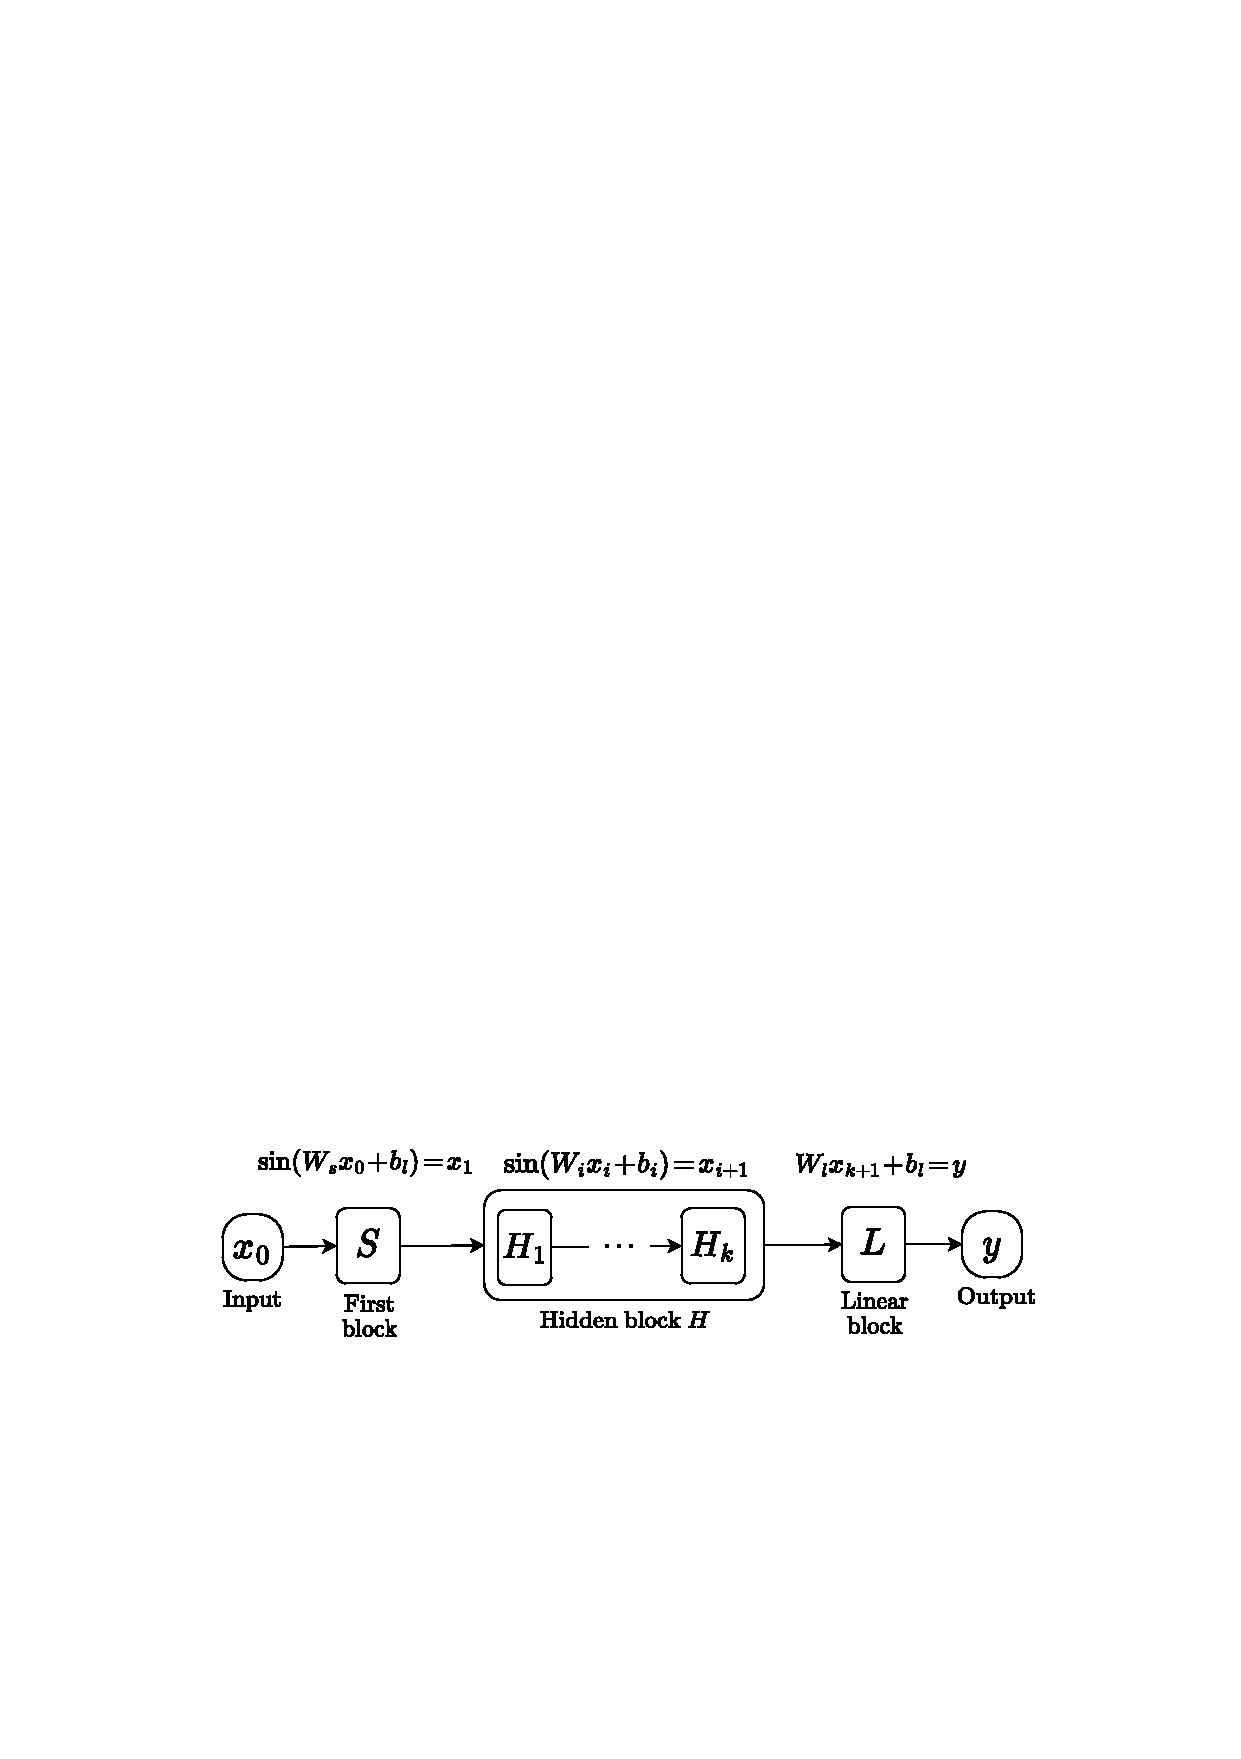
\includegraphics[width=0.9\linewidth]{img/ch4/diagram_mr_module.pdf}
    \caption{General Anatomy of a MR-Module.}
    \label{f:mr-module}
\end{figure}

The specific choice and configuration of these layers define the two types of MR-Modules: \textbf{Pure Sine MR-Module}, a shallow MLP with only the sinusoidal layer \( S \) and linear layer \( L \); and \textbf{Modulated Sine MR-Module}, a deep MLP that includes one or more hidden layers \( H \).

At the end of each level, the control layer \( c_i(t) \) regulates the blending of the MR-Modules, enabling continuous transitions between different resolution stages.

\subsubsection{Pure Sine MR-Module}

The \textit{Pure Sine MR-Module} is a shallow sinusoidal multi-layer perceptron (MLP) that acts as a basic spectral filter. It is defined as the composition \( L \circ S \) of a sinusoidal layer \( S \), followed by a linear output layer \( L \).

The sinusoidal layer \( S\!:\!\mathbb{R}^d\!\to\! \mathbb{R}^m \) projects the input \( x \in \mathbb{R}^d \) into a dictionary of \( m \) sines of the form \( S(x) = \sin\left(W_s x + b_s\right) \), where \( W_s \in \mathbb{R}^{m \times d} \) is a weight matrix and \( b_s \in \mathbb{R}^m \) is a bias vector. The integer \( m \) is referred to as the \textit{width} of the MR-Module, determining the number of sinusoidal basis functions used. The linear layer \( L\!:\!\mathbb{R}^m\!\to\! \mathbb{R}^n \) is an affine map defined as \( L(x) = W_l x + b_l \), where \( W_l \in \mathbb{R}^{n \times m} \), \( b_l \in \mathbb{R}^n \), and $n$ is the dimension of the output vector.

As discussed in Chapter \ref{chap:sinusoidal}, this architecture behaves as a spectral filter because the initialization of \( W_s \) directly determines the range of frequencies that the MR-Module can capture. Thus, \( W_s \) effectively defines the spectrum of frequencies the module is capable of learning, making the module's performance more sensitive to the initial configuration of the sine functions.

Figure \ref{f:pure-sine} illustrates the structure of a Pure Sine MR-Module and provides an example of a signal represented as a linear combination of two frequencies. In this example, the sinusoidal layer is defined as \( S(x) = (\sin(x), \sin(5x)) \) and the linear layer simply sums the two outputs, \( L(x_1, x_2) = x_1 + x_2 \).

\begin{figure}[!h]
\centering
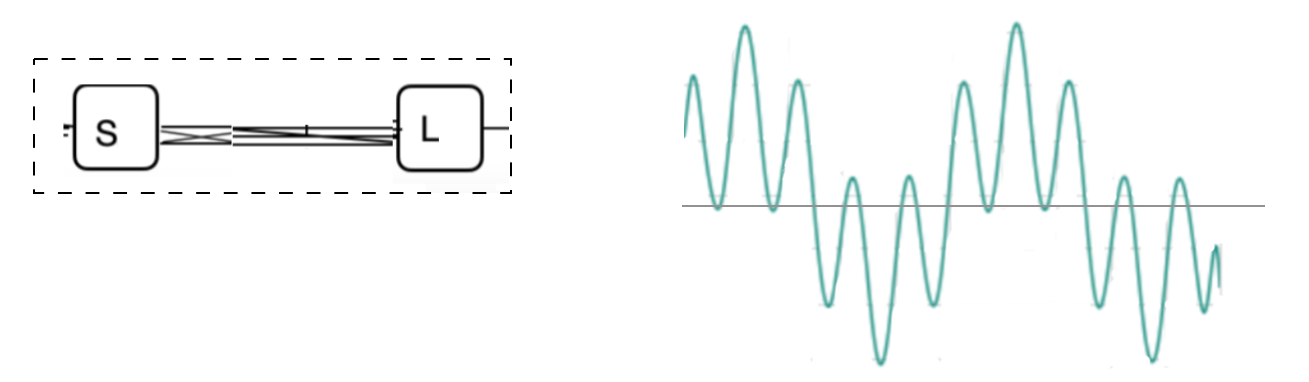
\includegraphics[width=0.8\linewidth]{img/ch4/pure-sine.png}
\caption{Pure Sine MR-Module: Network structure and an example signal formed by a linear combination of two frequencies.}
\label{f:pure-sine}
\end{figure}

\subsubsection{Modulated Sine MR-Module}

The \textit{Modulated Sine MR-Module} extends the capacity of the Pure Sine MR-Module by incorporating additional nonlinear transformations through a deep sinusoidal block. It is defined as a composition \( L \circ H \circ S \), where \( S \) is a sinusoidal layer, \( H \) is a hidden block of multiple sinusoidal transformations, and \( L \) is a linear output layer.

The hidden block \( H\!:\!\mathbb{R}^m\!\to\! \mathbb{R}^m \) is a composition of \( k \) sinusoidal layers, expressed as \( H = H_k \circ \cdots \circ H_1 \), where each layer \( H_i(x_i) = \sin\left(W_i x_i + b_i\right) \) produces the input for the next layer, with \( x_0 \in \mathbb{R}^m \) serving as the input to the hidden block. The parameters \( m \) and \( k \) determine the \textit{width} and \textit{depth} of the MR-Module, respectively. The output layer \( L \!:\! \mathbb{R}^m \!\to\! \mathbb{R}^n \) functions similarly to the linear layer in the Pure Sine MR-Module.

This deeper architecture has several implications. First, the Modulated Sine MR-Module has a higher representational capacity than its shallow counterpart for the same number of neurons, due to the hierarchical composition of sine functions \citep{novello2022understanding}. Second, its frequency response is not straightforwardly controlled by the initial weights of \( W_s \), as the nested sinusoidal layers \( H \) create a more complex, nonlinear mapping.


Figure \ref{f:modulated} illustrates a Modulated Sine MR-Module and an example of a nested sinusoidal function \( \sin\left( 3\sin\left(5\sin(1.9x)\right)\right) \), showcasing its ability to approximate complex frequency compositions. In this example, the initial sinusoidal layer is \( S(x) = \sin(1.9 x) \), the hidden block is \( H(x) = \sin\left(3\sin(5x)\right) \), and the output layer is simply the identity function \( L(x) = x \). Note that the resulting spectral atoms, i.e., the output functions of \( H \circ S \), can adapt to fit local variations of the input signal's frequencies, enabling a semi-local representation of the signal in both space and frequency domains.

\begin{figure}[!h]
\centering
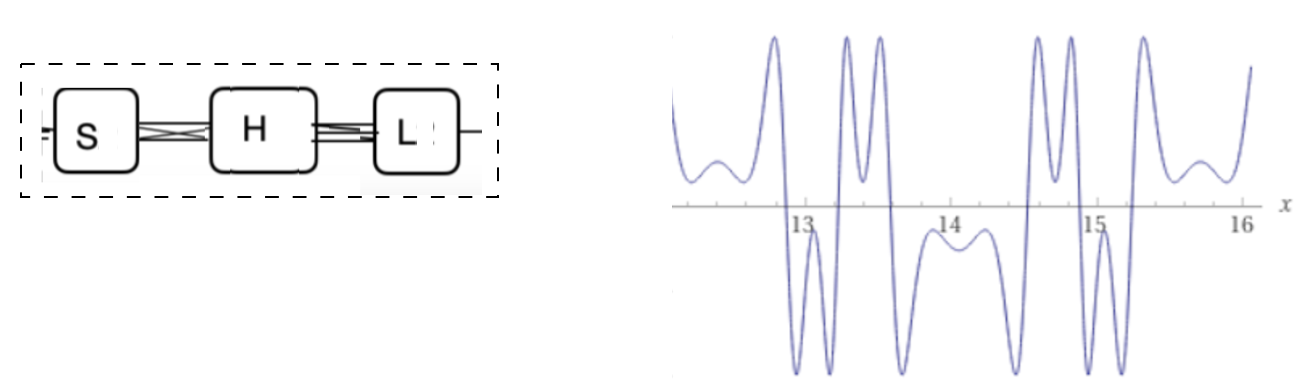
\includegraphics[width=0.9\linewidth]{img/ch4/modulated-sine.png}
\caption{Modulated Sine MR-Module: Network structure and an example of a nested sinusoidal function.}
\label{f:modulated}
\end{figure}

By combining these two types of MR-Modules at different stages of the MR-Net, we can control the approximation of details with varying levels of complexity.


\section{MR-Net Subclasses}

In this section, we define three subclasses of the MR-Net, namely, the \textbf{S-Net} (Shallow Network), \textbf{L-Net} (Laplacian Network), and \textbf{M-Net} (Modulated Network), which vary in complexity and representational power depending on the configuration of their stages. Recall from Equation \ref{e-mrnet} that a MR-Net is a function \( f : \mathbb{R}^d \times [0, N] \to \mathbb{R}^n \) defined as a weighted sum of \( N \) individual stages:

\[
f(x, t) = c_0(t)g_0(x) + \cdots + c_{N-1}(t)g_{N-1}(x).
\]

Each stage \( g_i \) corresponds to a neural module that approximates a portion of the target signal at a specific resolution. To specify the subclasses S-Net, L-Net, and M-Net, we configure the internal structure of these stages using different types of sinusoidal MR-Modules, as described below.

\subsection{S-Net: Shallow Sine Stages}

The S-Net is the simplest form of MR-Net, where each stage \( g_i \) is constructed using a pure sine MR-Module. That is, \( g_i = L_i \circ S_i \), where \( S_i \) and \( L_i \) are the first and linear layers, respectively, of the sinusoidal network. Since \( g_i \) is a shallow module, it can be expressed directly as a sum of sine functions:

\begin{align}
    g_i(x) = a_0 + \sum_{j=1}^m a_j \sin\left(\omega_j x + \varphi_j\right),
\end{align}


where the \textit{frequencies} \( \omega_j \) and \textit{phase shifts} \( \varphi_j \) are defined by the weights and biases of the sinusoidal layer \( S_i \). The \textit{amplitudes} \( a_j \) are given by the linear layer \( L_i \).

This structure allows each stage \( g_i \) to serve as a basic spectral filter that captures different frequency components of the input signal. Consequently, the S-Net can control its level of detail by adjusting the frequency bands of each stage. The overall architecture of the S-Net is illustrated in Figure \ref{f:s-net}.

\begin{figure}[!h]
\centering
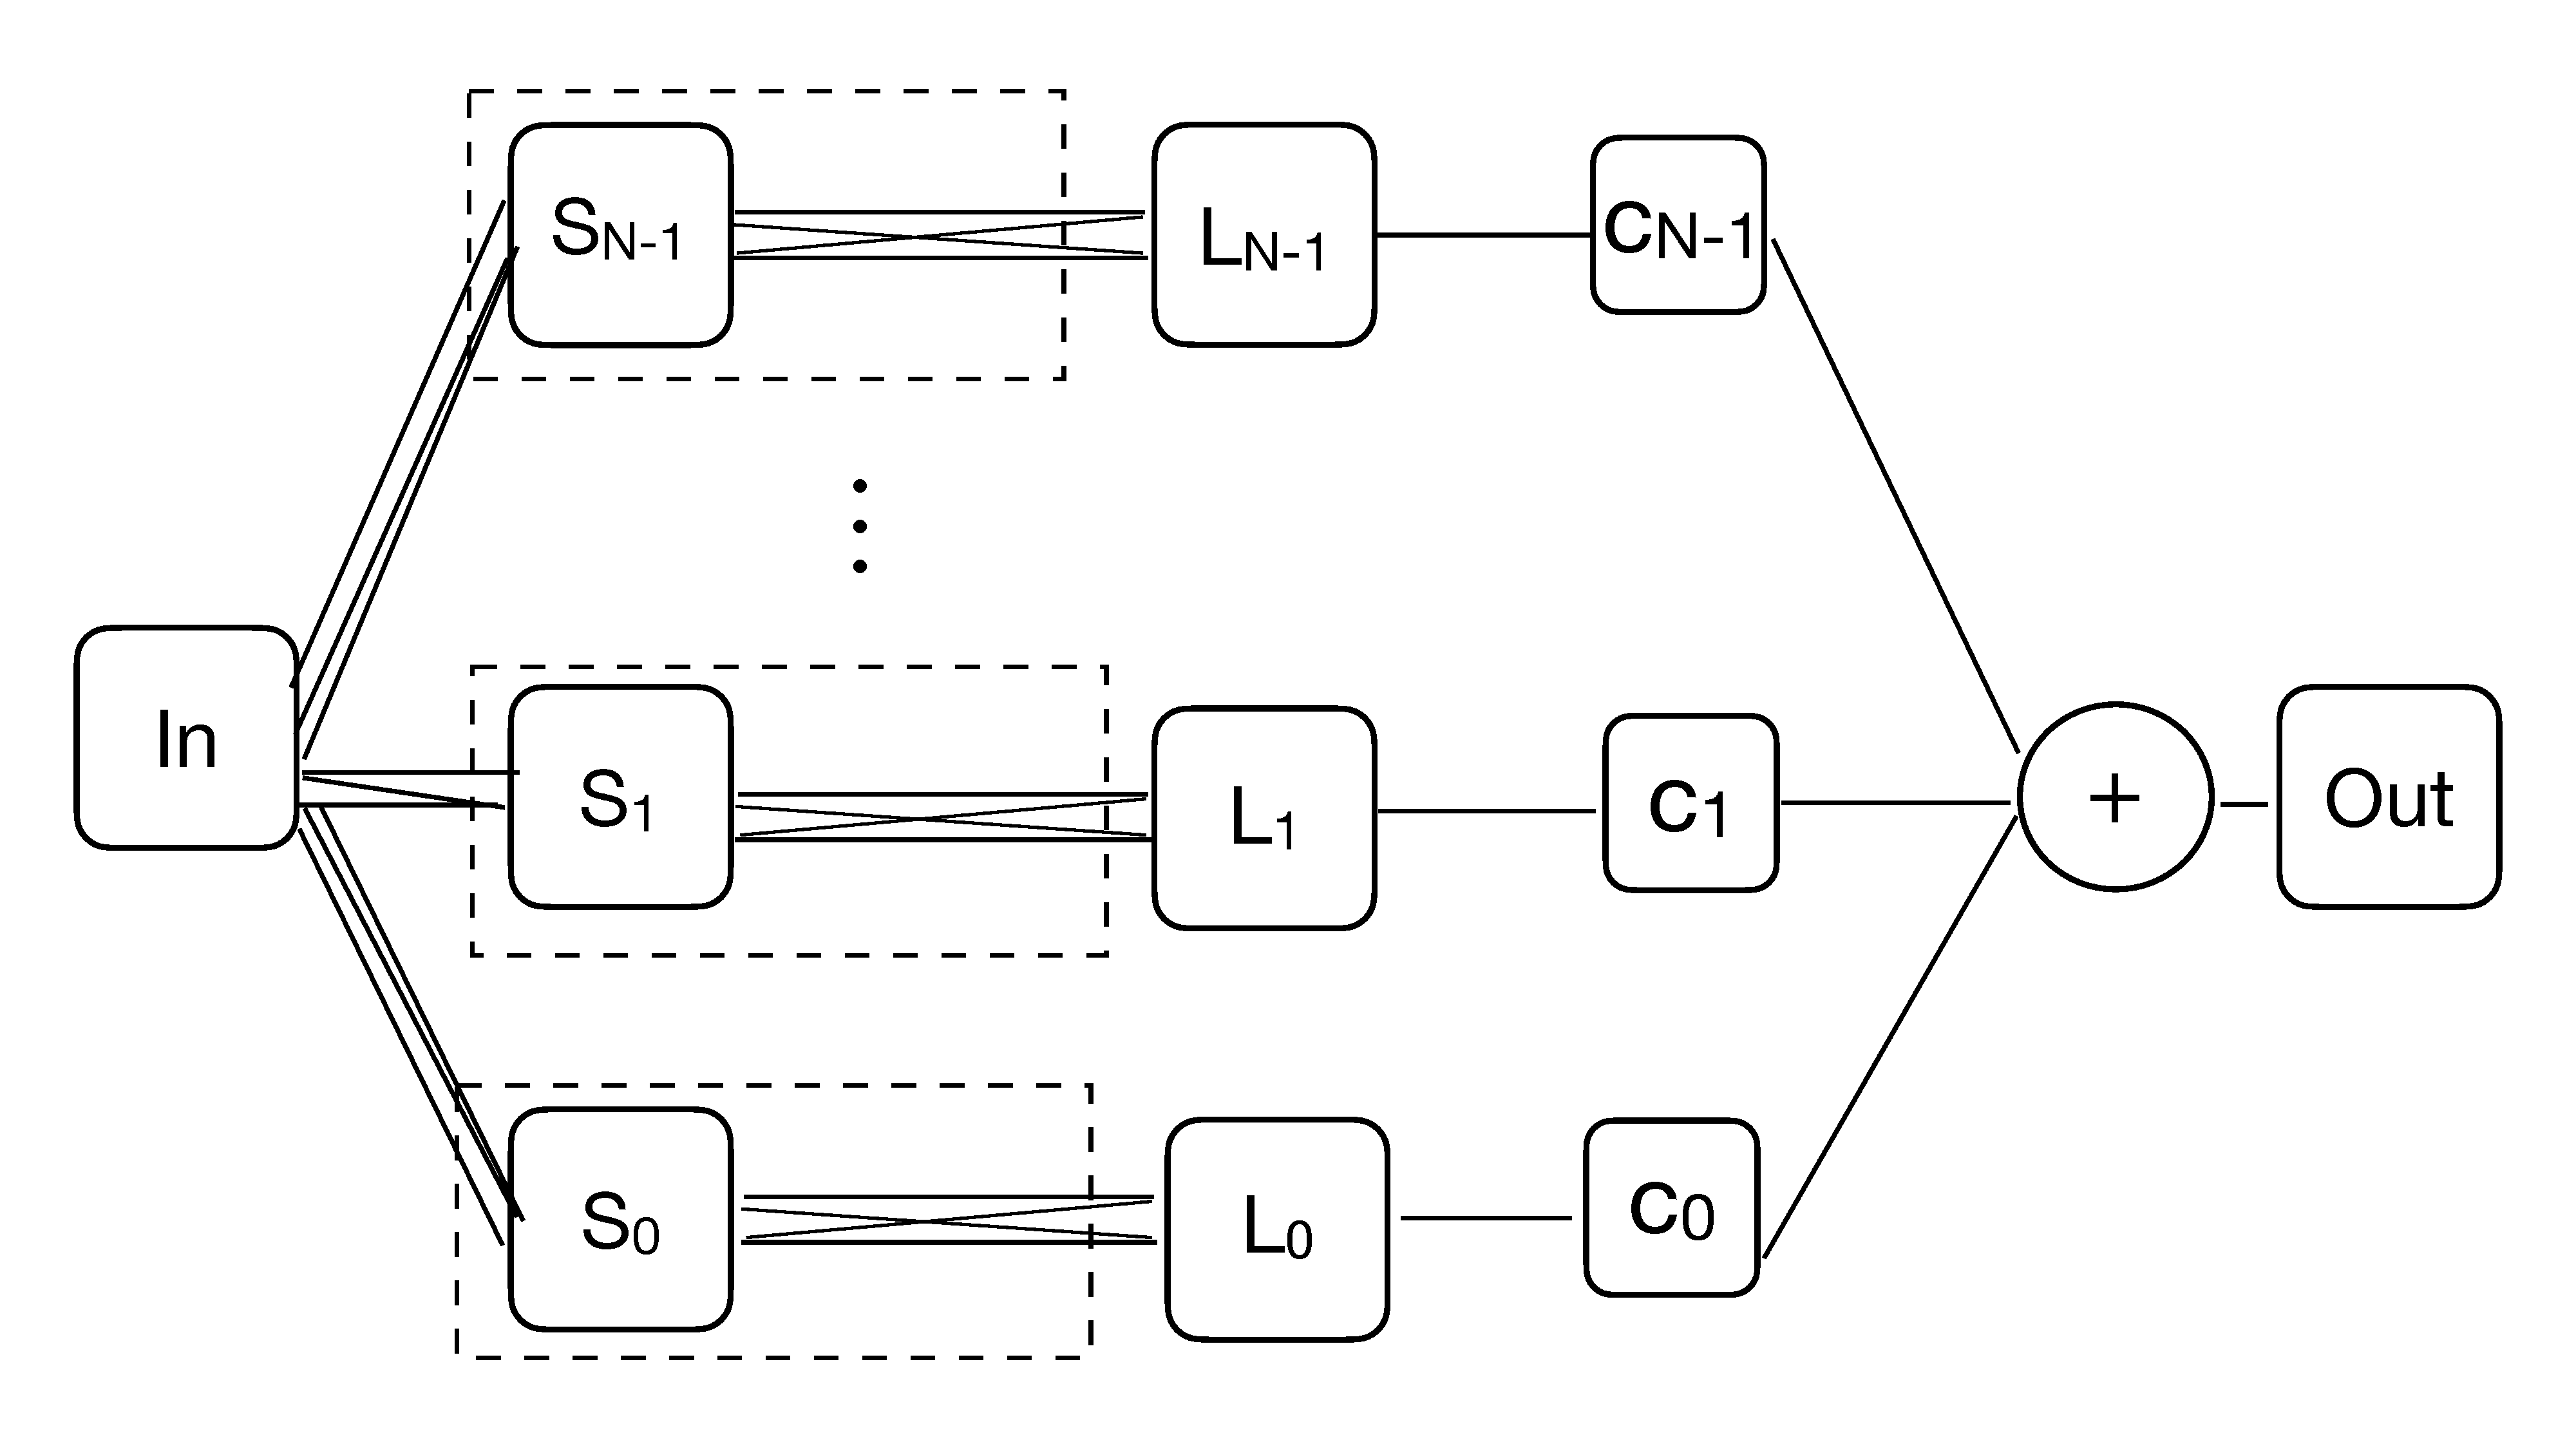
\includegraphics[width=0.58\linewidth]{img/ch4/snet.pdf}
\caption{S-Net architecture: Each stage is a pure sine MR-Module acting as a localized spectral filter.}
\label{f:s-net}
\end{figure}

\subsection{L-Net: Independent Modulated Sine Stages}
\label{s-lnet}

The L-Net extends the S-Net by using a deeper module for each stage \( g_i \). In this configuration, each stage is a modulated sine MR-Module defined as \( g_i = L_i \circ H_i \circ S_i \), where \( S_i \), \( H_i \), and \( L_i \) are the sinusoidal, hidden, and linear layers, respectively (see Fig.~\ref{f:l-net}).

\begin{figure}[!h]
    \centering
    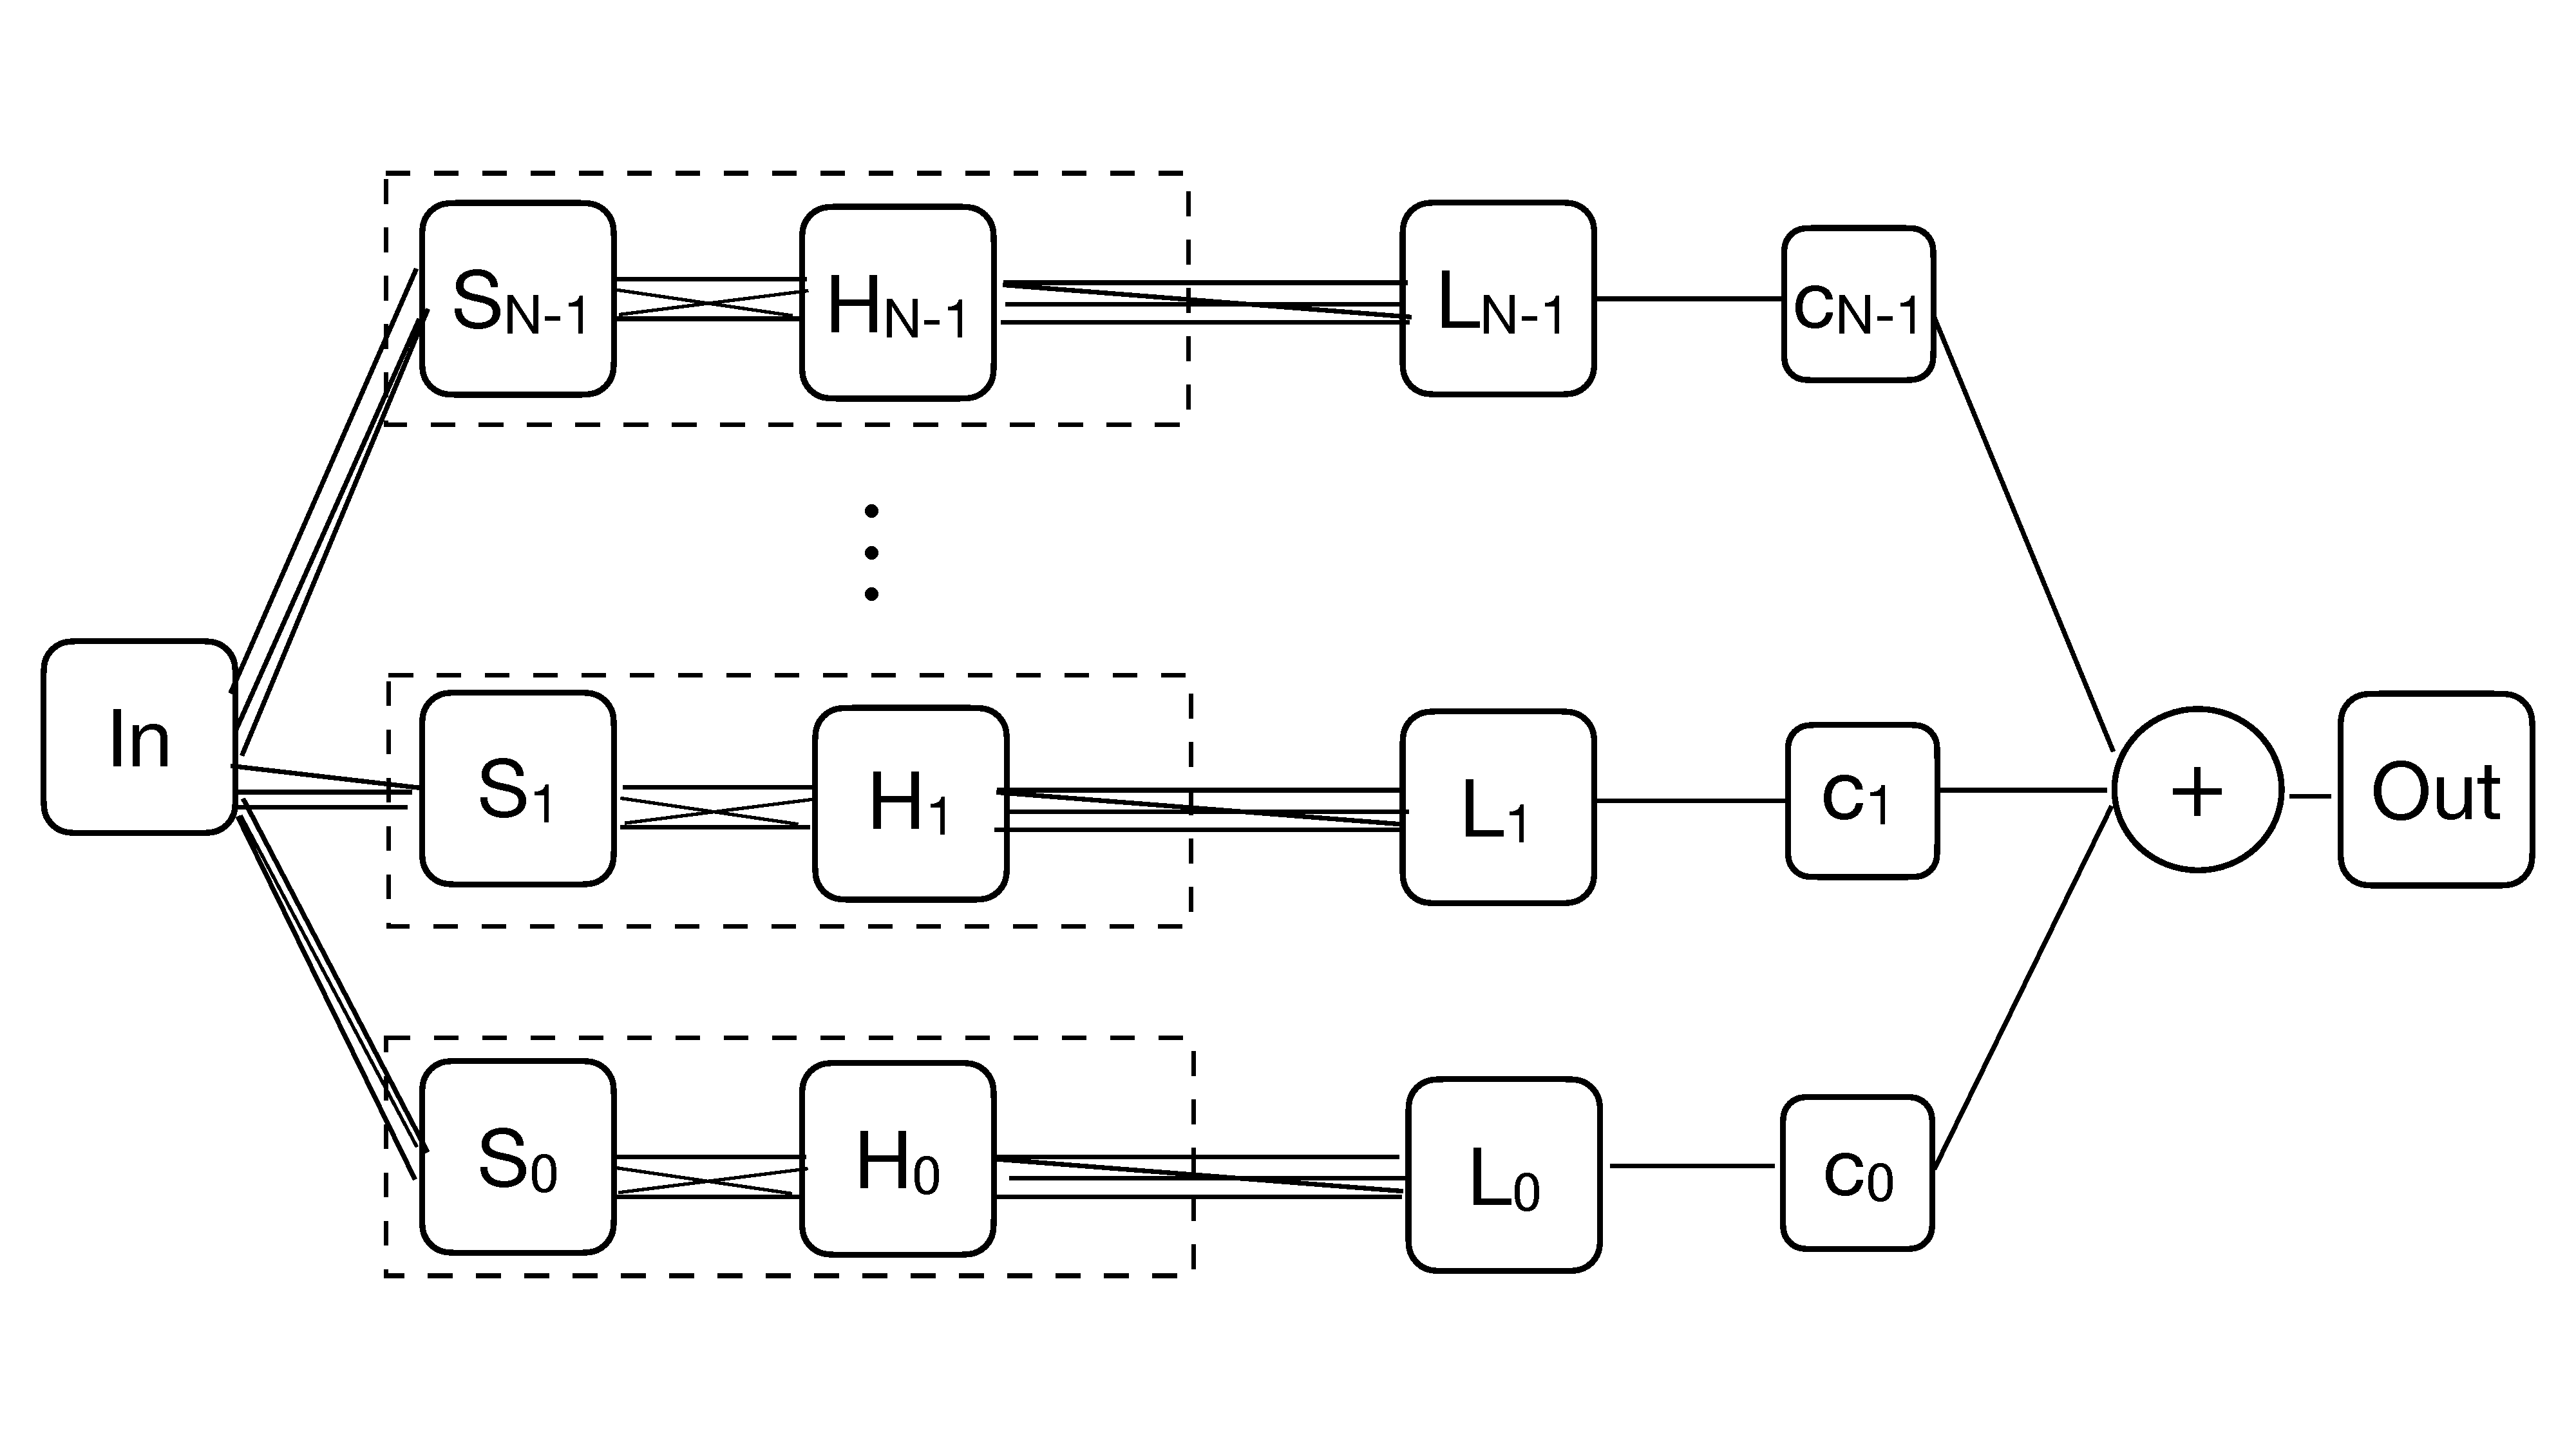
\includegraphics[width=0.7\linewidth]{img/ch4/lnet.pdf}
    \caption{L-Net architecture: Each stage is an independent modulated sine MR-Module, allowing for increased complexity and expressiveness.}
    \label{f:l-net}
\end{figure}

The key difference in the L-Net is the increased expressiveness due to the added depth of each stage. By incorporating the hidden block \( H_i \), each stage can model more complex compositions of sinusoidal functions, allowing the L-Net to capture finer details of the input signal quicker. As a result, the overall level of detail depends on the width and depth of the hidden block in each stage. 


An interesting property of the L-Net is that when considering the final stage at level \( N \), the function \( f(\cdot, N) \) \textit{behaves like a single deep sinusoidal} MLP. Without loss of generality, let \( f(x, t) = c_0(t)g_0(x) + c_1(t)g_1(x) \) be a two-stage L-Net with the same architecture for each stage, with a single hidden layer. Then, at \( t = 2 \), we show that the L-Net can be represented as \( f(x, 2) = L \circ H \circ S \), where \( L \), \( H \), and \( S \) combine the corresponding matrices of the stages. For this, define the matrices of $S$, $H$, and $L$, respectively, using $W_s\!=\!\begin{psmallmatrix}W_s^0\\W_s^1\end{psmallmatrix}$, 
$W_h\!=\!\begin{psmallmatrix}W_h^0& 0\\0&W_h^1\end{psmallmatrix}$, 
$W_l\!=\!\begin{psmallmatrix}W_l^0 & W_l^1\end{psmallmatrix}$, where $W_s^j$, $W_h^j$, $W_l^j$ are the matrices of the stages~$g_j$. The biases are defined similarly. This process generalizes to any \( N \)-stage L-Net in an analogous way, providing a controllable method to increase the effective \textit{width} of a sinusoidal MLP.

\subsection{M-Net: Hierarchical Modulated Stages}
\label{s-mnet}

Unlike the S-Net and L-Net, in which the stages are independent of each other, the M-Net introduces a hierarchical structure that reuses information learned at earlier stages. In the M-Net, each stage \( g_i \) is a modulated sine MR-Module that is \textit{directly linked to the subsequent stage} \( g_{i+1} \) through its hidden block as illustrated in Figure \ref{f:m-net}.

\begin{figure}[!h]
    \centering
    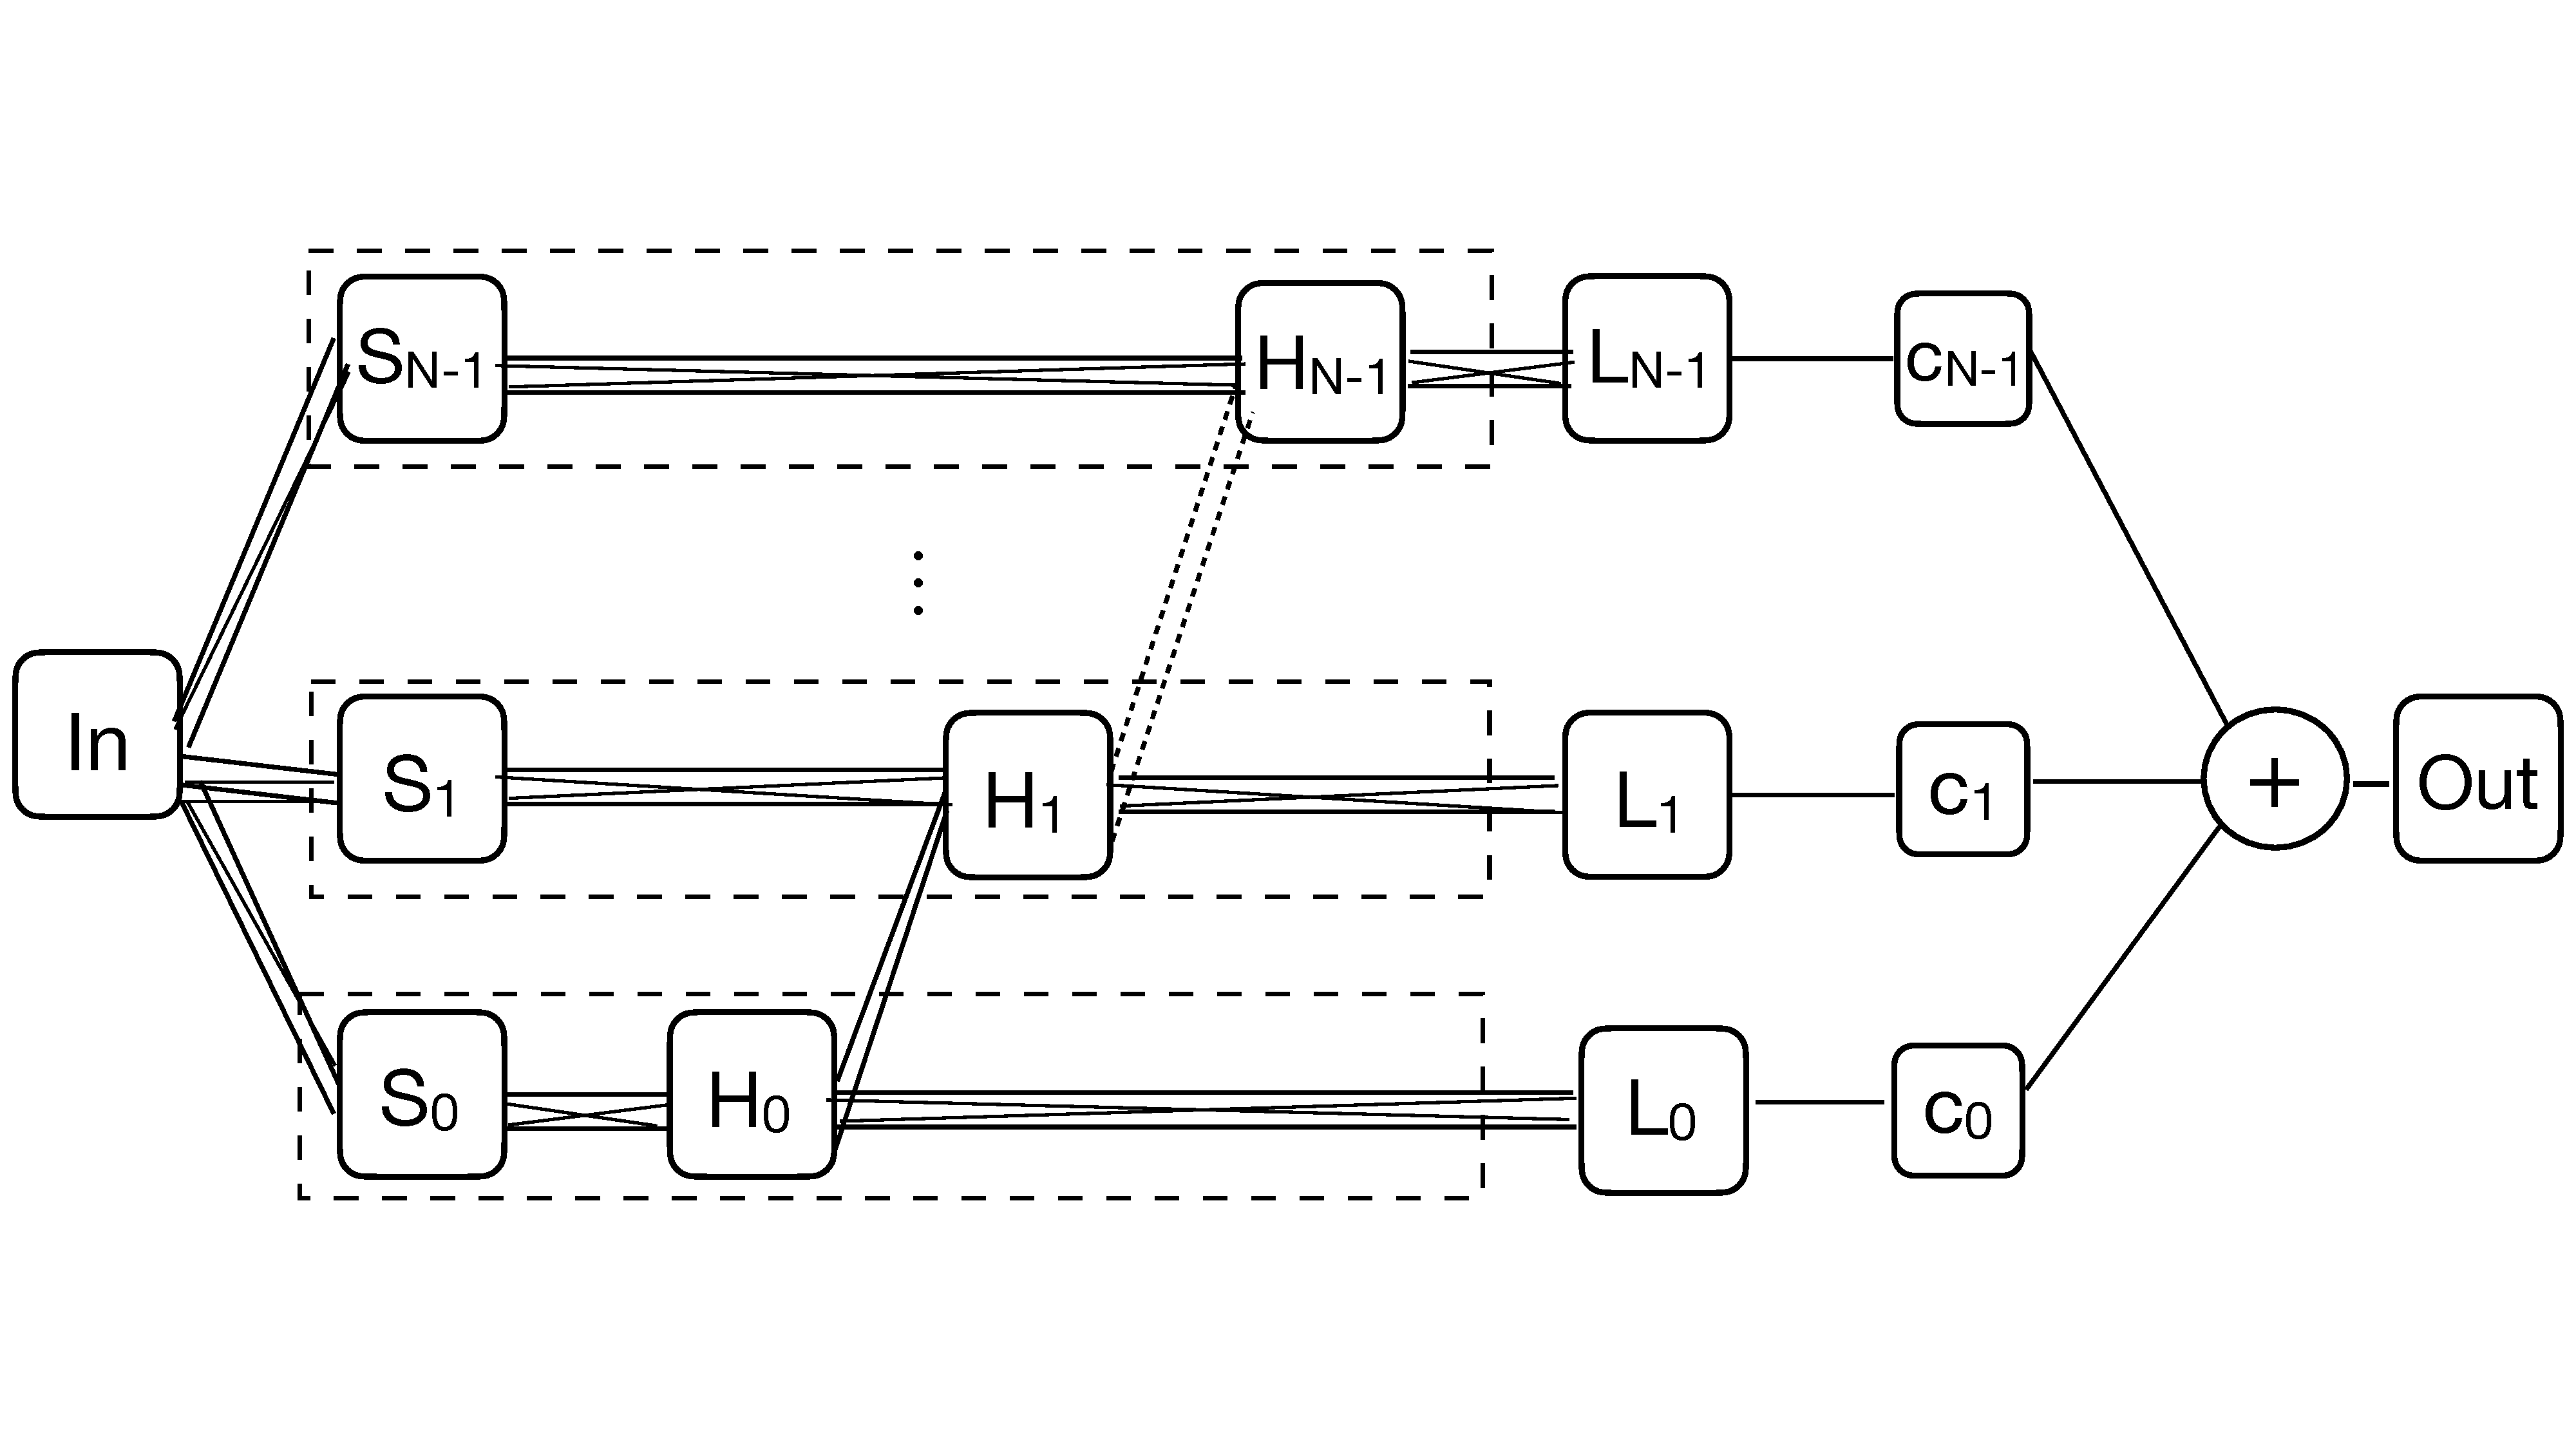
\includegraphics[width=0.75\linewidth]{img/ch4/mnet.pdf}
    \caption{M-Net architecture: Hierarchical connection between hidden layers allows for reuse of information and progressively refined representations.}
    \label{f:m-net}
\end{figure}
    
Specifically, $H_i\circ  S_i$ is composed both with the linear layer $L_i$, producing the stage $g_i\! =\! L_i\!\circ\! H_i\!\circ\!  S_i$, and the hidden block $H_{i+1}$ resulting in $g_{i+1}\! =\! L_{i+1}\!\circ H_{i+1}\!\circ\left(S_{i+1}, H_i\circ  S_i\right)$. This way, the the hidden block has the form $H_{i+1}\!:\!\R^{m_{i+1} + m_i}\!\to\! \R^{m_{i+1}}$; $m_i$ is the dimension of the output of the last hidden layer of stage $i$. 

This sequential linkage creates a hierarchical representation in which each stage can build upon and refine the features captured by previous stages. Considering the following notation:

\begin{align}
    \overline{H_k} = H_k \circ (\overline{H_{k-1}}, S_{k}), \\
    \overline{H_0} = H_0 \circ S_0
\end{align}

Each stage $g_i$ of the M-Net can thus be viewed as a deep sinusoidal MLP like:

\begin{align}
    g_0 = L_0 \circ H_0 \circ S_0 \\
    g_1 = L_1 \circ H_1 \circ (H_0 \circ S_0, S_1) = L_1 \circ H_1 \circ (\overline{H_0}, S_1)\\
    &\vdots\\
    g_{N-1} = L_{N-1} \circ H_{N-1} \circ (\overline{H_{N-2}}, S_{N-1}),
\end{align}

where the overall M-Net is obtained by adding the stages according to Equation \ref{e-mrnet}.

% where \( \overline{H_i} \) represents the part of \( H_i \) that connects to stage \( g_{i+1} \).

This architecture provides a controllable way to increase the effective \textit{depth} of the sinusoidal MLP during training, making the M-Net particularly suitable for applications requiring compact multiresolution representations (see Section \ref{sec:considerations}).


\section{Multiresolution Training}\label{sec:mr_training}
\label{s:training}

The training of the MR-Net $f$ is inherently aligned with the hierarchical nature of its architecture, where each stage $g_i$ should contribute in representing a specific level of detail in the target signal $\gt{f}$. The training process typically follows a sequential, stage-wise approach, starting with the lowest-frequency stage and gradually incorporating higher-frequency stages. This learning strategy allows MR-Net to build a comprehensive representation of the signal, beginning with coarse features and progressively refining the model with finer nuances. To maintain the integrity of the multiresolution representation, once a stage is trained to capture its designated level of detail, its parameters are "frozen". This freezing process preserves the learned coarse features while subsequent stages focus on refining finer details. By doing so, the network prevents overwriting of information already captured in earlier stages, ensuring a stable and consistent multiresolution representation throughout the training process.

The MR-Stages $\{g_i\}$ are the building blocks of the MR-Net $f$. They form a stack of MR-Modules that are interconnected according to the specific MR-Net subclass. The representational capacity of each stage $g_i$ can be fine-tuned by initializing its first layer to specific frequencies, adjusting the depth and width of the network, or incorporating ground-truth values $\gt{g}_i$ during training. The overall MR-Net configuration is defined by the parameters of its stages, including the number of stages, as well as the depth and width of each stage.

The MR-Net training process offers flexibility in terms of signal processing. Depending on the desired frequency characteristics for each stage, the input to MR-Net can either 
be the original ground-truth signal or a low-pass filtered version, supporting diverse multiresolution schemes. As each stage is trained, it uses an adaptive loss functional that compares the network's output at that particular stage with the corresponding level of detail in the ground truth signal. In this section we describe each of the components in the training process in detail.

\subsection{Input Data}

Each MR-Net stage \( g_i \) is trained using pairs of samples \(\{x_j, y_j\}\), where \( x_j \) are points sampled from the domain \(\mathcal{D}\) of the ground-truth function \(\gt{f}\), and \( y_j = \gt{f}(x_j) \in \mathcal{C} \) are the corresponding values in the codomain. For example, for a square image, the domain could be defined as \(\mathcal{D} = [-1, 1]^2 \subset \mathbb{R}^{2}\). Note that spatial media objects, such as images or 3D models, may be embedded in any region of their respective spaces. This image signal \(\gt{f}\) could have codomains in a monochromatic space (\(\mathcal{C} = \mathbb{R}\)) or a trichromatic color space (\(\mathcal{C} = \mathbb{R}^3\)) as the RGB. Depending on the application, alternative color spaces or additional attributes, such as segmentation masks or feature maps (Figure \ref{f:ex-signal-attributes}), may also be used. These additional attributes will be explored further in Chapter \ref{chap:seamless-textures}. 
% Figure \ref{f:ex-signal-attributes} illustrates examples of these attributes.

\begin{figure}[h]
    \centering
    \begin{subfigure}[b]{0.24\textwidth}
        \centering
        
\includegraphics[width=\textwidth]{img/ch4/sloth.jpg}
        \caption{RGB \newline \centering values}
    \end{subfigure}
    \begin{subfigure}[b]{0.24\textwidth}
        \centering
        
\includegraphics[width=\textwidth]{img/ch4/grayscale.png}
        \caption{Monochromatic}
    \end{subfigure}
    \begin{subfigure}[b]{0.24\textwidth}
        \centering
        
\includegraphics[width=\textwidth]{img/ch4/mask.png}
        \caption{Mask \newline}
    \end{subfigure}
    \begin{subfigure}[b]{0.24\textwidth}
        \centering
        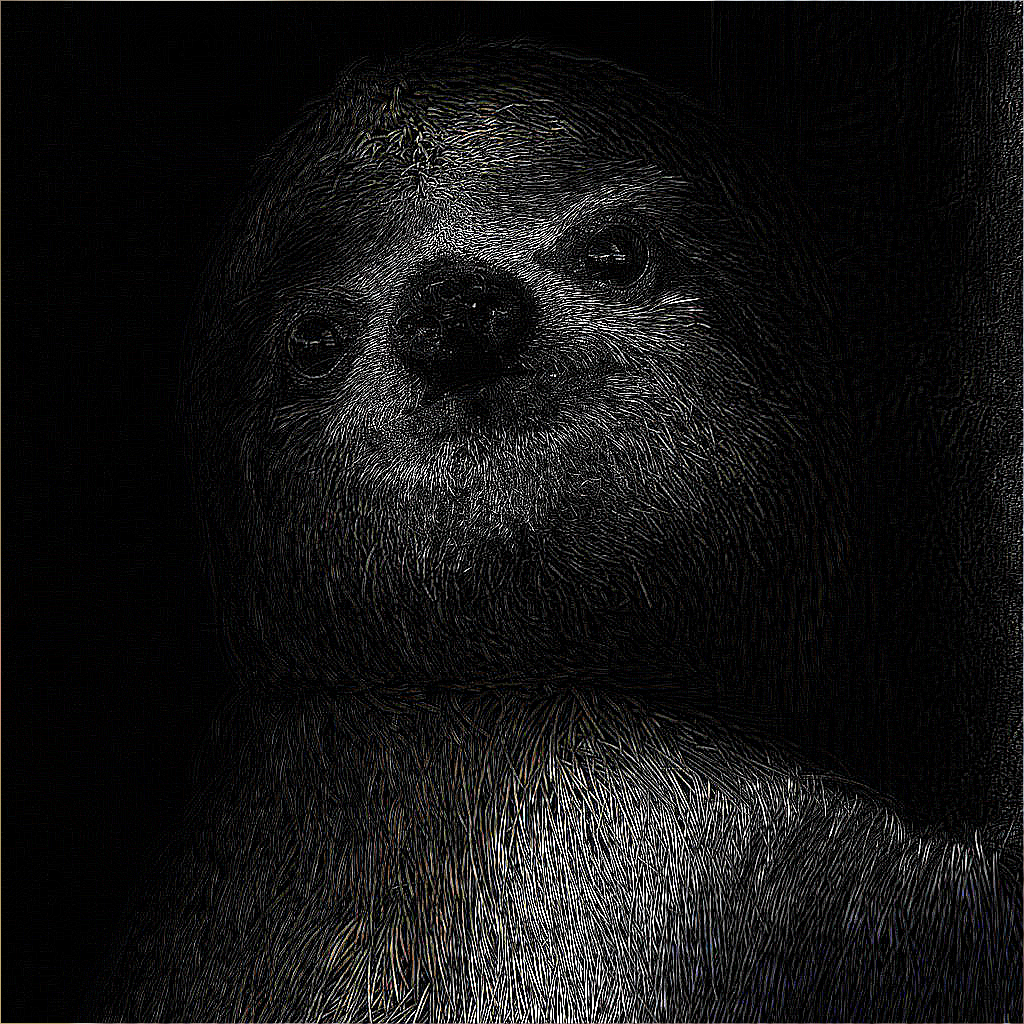
\includegraphics[width=\textwidth]{img/ch4/edges.png}
        \caption{Edges \newline}
    \end{subfigure}
    \caption{Example of attributes and features that can be used in training}
    \label{f:ex-signal-attributes}
\end{figure}

For the training of each of the \( N \) stages \( g_i \), the input data is organized into a \textit{multi-stage stack} \(\{x_j, y_j\}_i\). Specifically, for each \( i \), the set of pairs \(\{x_j, y_j\}_i\) represents samples from either the \( i \)-th level of detail \(\gt{f}_i\) of the signal \(\gt{f}\), or from the original signal \(\gt{f}\) itself, with \(\{x_j\}_i \subset \mathcal{D}\) and \(\{y_j\}_i = \{\gt{f}_i(x_j)\}\). The choice of sampling strategy to generate the multi-stage stack \(\{x_j, y_j\}_i\) from the signal \(\gt{f}\) is an important consideration in the MR-Net training.


\subsubsection{Sampling Strategies}

There are two primary sampling strategies: \textit{regular} and \textit{irregular} sampling. In this work, we focus on regular sampling, also known as uniform sampling, which is more commonly used and is supported by a well-established theoretical foundation for sampling and reconstruction. However, Chapter \ref{chap:future} will touch on some intriguing possibilities for irregular sampling and areas where it could offer future research opportunities.

In regular sampling, the points are arranged in a uniform grid \(\{x_{k,l}\}\) that discretizes the domain \(\mathcal{D}\). From the perspective of \textit{representation theory}, this setup can be interpreted as projecting the function \(\gt{f}_i\) onto the primal \textit{Shannon basis} (i.e., a grid of Dirac delta distributions). In signal processing terms, this basis is a grid of impulses, and the function is represented as the sequence \(\{y_j\}_i\) at corresponding grid locations \(\{x_j\}_i\).

At the highest resolution, the points form a square grid of size \( 2^k \) for some integer \( k > N \). The multi-stage grids \(\{x_{k,l}\}_i\) follow a dyadic lattice structure governed by the \( 2^i \) rule:

\begin{align}
    \{x_{k,l}\}_i = \{x_{2k, 2l}\}_{i+1}, \quad \text{where} \quad \{x_{k,l}\}_N = \{x_{k,l}\}.
\end{align}


This formulation ensures that each dimension of the grid \(\{x_{k,l}\}_i\) has twice the size of the previous stage grid, forming a pyramid structure (see Figure~\ref{f:multi}(a)).

Alternatively, we can consider a fixed resolution for the sampling grids \(\{x_{k,l}\}_i\), where the signal \(\gt{f}\) is sampled at its highest level, or directly at the level of detail \(\gt{f}_i\) for each stage grid \(\{x_{k,l}\}_i\) (see Figure~\ref{f:multi}(b)). More details about this approach are provided in Section~\ref{s:lod}.

\begin{figure}[!h]
\centering
\begin{subfigure}{0.45\linewidth}
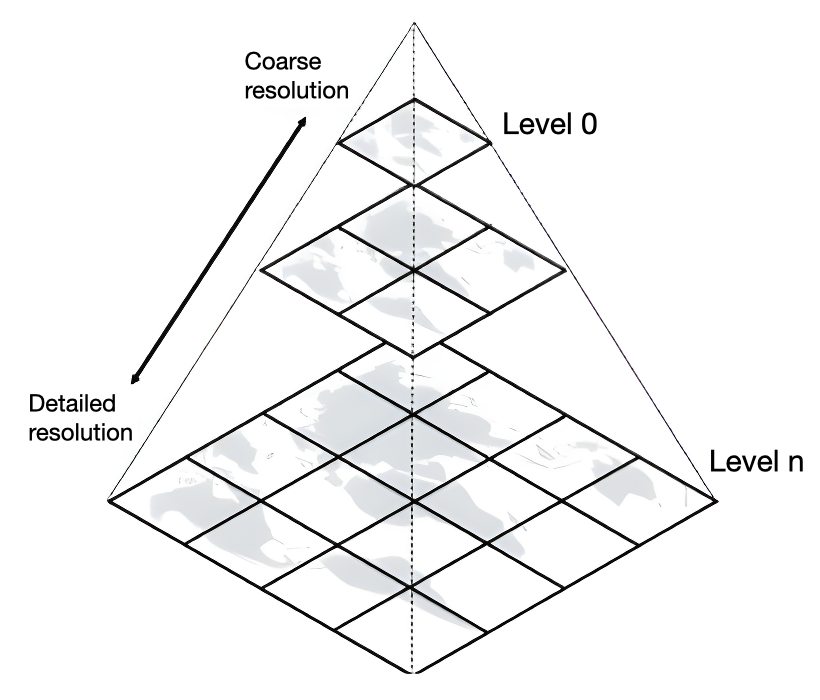
\includegraphics[width=\linewidth]{img/ch4/pyramid.png}
\caption{Pyramid Configuration}
\end{subfigure}
\begin{subfigure}{0.45\linewidth}
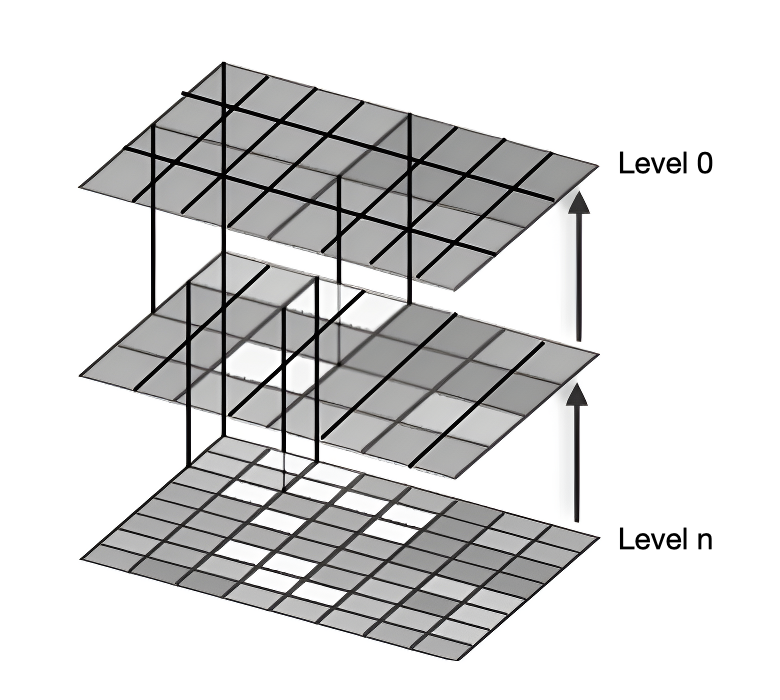
\includegraphics[width=\linewidth]{img/ch4/tower.png}    
\caption{Tower Configuration}
\end{subfigure}
\caption{Examples of multi-stage stack configurations.}
\label{f:multi}
\end{figure}

\subsubsection{Filtering Strategies}

Each level $i$ of the multi-stage stack can be filtered to separate specific frequency bands from the level of detail $\gt{f}_{i+1}$. In this context, we can use different variations of the signal \(\gt{f}\) for the stages, such as the unfiltered signal, a low-pass filtered version of \(\gt{f}_{i+1}\), or a band-pass filtered version of \(\gt{f}_{i+1}\). Usually, a Gaussian kernel is used for low-pass filtering, while a difference of Gaussians (DoG) kernel is used for band-pass filtering (see Figure~\ref{f:filter}).

The filtering operation for a low-pass version of stage \(\gt{f}_{i+1}\) is defined by convolving it with a Gaussian kernel \( K \):

\begin{align}\label{e-gaussian-filter}
    \gt{f}_i(k,l) &= \left( K * \gt{f}_{i+1} \right)(k, l).
\end{align}

We slighly abuse the notation by denoting $\gt{f}_i(k,l)$ as the function $\gt{f}_i$ evaluated at the point $x_{k,l}$. Similarly, the band-pass filtered stage \(\gt{g}_i\) is defined as the difference between the stage \(\gt{f}_i\) and its low-pass filtered version:

\begin{align}
    \gt{g}_i(k,l) = \left( \gt{f}_{i} - K * \gt{f}_{i} \right)(k, l).
\end{align}

\begin{figure}[!h]
    \centering
    
\includegraphics[width=0.28\linewidth]{img/ch4/grayscale.png}
    
\includegraphics[width=0.28\linewidth]{img/ch4/blurred.png}
    
\includegraphics[width=0.28\linewidth]{img/ch4/dog.png}\\
    {\hfil \hfil signal \hfil \hfil \hfil low-pass \hfil \hfil \hfil band-pass \hfil}
    \caption{Examples of different filter types.}
    \label{f:filter}
\end{figure}

% \pagebreak

\subsection{Level of Detail Schemes}
\label{s:lod}

By integrating the concepts introduced in the previous section, we can establish various strategies for learning level-of-detail representations using MR-Nets. The main schemes explored here are: Capacity-Based with Original Signal; Filtering with Gaussian/Laplacian Tower; and Filtering with Gaussian/Laplacian Pyramid.

\subsubsection{Capacity Based with Original Signal}

In this scheme, we train each stage $g_i$ of the MR-Net $f$ on the same sampling of the ground-truth signal $\gt{f}$, which is assumed to have no frequencies higher than a defined bandlimit $\omega$. The multi-stage stack $\{x_j, y_j\}_i$ used as input is composed of $N$ copies of the same sample $\{x_j, y_j\}$ of $\gt{f}$. As a result, \textit{every stage receives identical training data}, even if they vary in their ability to approximate the signal.

This approach leverages the fact that even when a sinusoidal neural network does not have enough capacity to perfectly reconstruct the ground-truth signal $\gt{f}$, it can still capture its lowest frequencies and reconstruct a smooth approximation of the signal when initialized appropriately, as discussed in Section \ref{sec:capacity-filtering}. 

The initialization of the $N$ stages $g_i$ of $f$ follows the scheme detailed in Section~\ref{sec:frequency-initialization}. We set the rows of the first matrix of each stage $g_i$ with values in $\Omega_i=[-\omega_i, \omega_i]^2$, where $\omega_i$ is a partition of the interval $[0,\omega]$ and $\omega$ is a frequency value based on the bandlimit of $\gt{f}$. Consequently, the first stage $g_0$ is configured to learn the lowest frequencies of $\gt{f}$ up to its capacity limit. As additional stages $g_1, g_2, \ldots, g_{N-1}$ are progressively added, they refine the learned representation by capturing more detail until the desired fidelity is achieved or the maximum number of stages is reached.

\subsubsection{Filtering with Gaussian / Laplacian Tower}

To gain more control over the frequencies present in the signal $\gt{f}$, we use a filtered multi-stage stack $\{x_j, y_j\}_i$, and train each MR-Net stage $g_i$ to approximate the corresponding level of detail \( \gt{f}_i \) from this stack.

We start by constructing a Gaussian tower, a multi-stage stack $\{x_j, y_j\}_i$ where each level $i$ is derived by applying a low-pass filter to the preceding level $i+1$. Specifically, the Gaussian tower $\{x_j, y_j\}_i$ is generated recursively by convolving the signal's level of detail $\gt{f}_i$ of $\gt{f}$ with a Gaussian kernel $K$:

\begin{align*}
    \gt{f}_i(x_j) &= \left(K * \gt{f}_{i+1}\right)(x_j), \\
    \gt{f}_{N-1} &= \gt{f}.
\end{align*}


At each level, the attribute $y_j$ is defined as $\gt{f}_i(x_j)$. Each stage $g_i$ of the MR-Net is trained using the corresponding level $i$ of the Gaussian tower, from the less detailed scale to the most detailed one. Note that each level is trained using the same amount of samples. Moreover, we aim to minimize the loss $\mathcal{L}_i = \norm{f_i(x_j)-y_j}^2$, where $f_i = g_0 + \dots + g_{i}$.

An alternative approach uses a Laplacian tower \( \{\gt{g}_i\} \), which isolates the \textit{residual detail} at each level:

\begin{align*}
    \gt{g}_i(x_j) &= \gt{f}_i(x_j) - \left(K * \gt{f}_i\right)(x_j), \\
    \gt{g}_0(x_j) &= \left(K * \gt{f}_1\right)(x_j).
\end{align*}

Here, $y_j = \gt{g}_i(x_j)$, and we train the MR-Net $f$ to minimize $\mathcal{L}_i = \norm{g_i(x_j)-y_j}^2$, where $g_i$ is the residual component at each stage.


\subsubsection{Filtering with Gaussian / Laplacian Pyramid}

Unlike the Gaussian tower, which is a highly redundant representation, the Gaussian pyramid is "critically sampled", meaning it uses the minimum number of samples necessary to represent each frequency band.

The Gaussian pyramid $\{x_{k,l}, y_{k,l}\}_i$ is constructed by recursively downsampling each level of the Gaussian tower of $\gt{f}$ by a factor of 2. Usually, the sampled points \( \{x_{k,l}\} \) form a grid of size \( 2^k \), for some integer $k$ greater than the number of levels in the pyramid. Each dimension of a grid $\{x_{k,l}\}_i$ is half the size of the previous stage's grid.

Similarly, the Laplacian pyramid is derived from the Laplacian tower by applying downsampling to the residual components, resulting in a compact, multiscale representation.
% Similarly, the \textit{Laplacian pyramid} is built using the Laplacian tower of $\gt{f}$, applying downsampling to the residual components.

% From the experiments in Section \ref{sec:generalization}, we conclude we can generalize correctly the model based only on the samples of a Gaussian pyramid. In terms of efficiency, it's faster to train the model on fewer samples, aligned with classical sampling theory results. This way, the Gaussian pyramid representation is more efficient and compact than the Gaussian tower. 

In Section~\ref{sec:generalization}, we demonstrate that it is possible to generalize the model using only the samples necessary to represent a certain frequency band. From that, we conclude that it is possible to train our network using a pyramid instead of a tower. From a computational standpoint, training the model with fewer samples is faster, an it is consistent with classical sampling theory. This way, the Gaussian pyramid offers a more efficient and compact representation for the multi-stage stack compared to the Gaussian tower.

When training on a multi-stage stack with grids of varying resolutions, it is possible to construct another multi-stage stack with the same resolution as the original signal for testing. In this case, the test data is constructed as a tower, where each level is filtered to match the corresponding level in the pyramid, separating the data into comparable frequency bands. With this preprocessing, the model is trained on the pyramid and evaluated on the full-resolution signal, comparing the results against the multi-resolution tower to assess generalization performance.

When training with a Gaussian/Laplacian pyramid, we initialize the stages $g_i$ of $f$ based on a dyadic sequence of frequency bands:

\[
\omega_{N-1}, \frac{\omega_{N-1}}{2}, \ldots, \frac{\omega_{N-1}}{2^{N-1}},
\]

where \( \omega_{N-1} \) is chosen based on the sampling rate of the highest resolution signal (see Section \ref{sec:frequency-initialization}). Each stage \( g_i \) is initialized with the frequency range \( \Omega_i = \left[-\omega_i, \omega_i\right]^2 \) for its first layer, ensuring that the network's frequency capabilities align with the pyramid structure and maintain the desired resolution properties.

% In practice, we assume that the data is given as a regular sample (digital image) of size $2^{k}\times 2^k$
% of the ground-truth signal~$\gt{f}$.
% We abuse the notation by denoting this digital image by~$\gt{f}$.
% To train the MR-Net stages~$\{g_i\}$, we use the (discrete) \textit{Gaussian} and \textit{Laplacian} pyramids of $\gt{f}$, both with $N<k$ levels.
% Precisely, the Gaussian pyramid $\{\gt{f}_i\}$ is defined recursively by convolving the \textit{level of detail} $\gt{f}_i$ with a Gaussian kernel $K$ and downsampling the result by a factor 2:
% \begin{align*}
%     \gt{f}_i(k,l)&=\left(K*\gt{f}_{i+1}\right)(2k,2l)\,\, \text{with} \,\, k,l\in \left\{1,\ldots, 2^{k-N+1+i}\right\},\\
%     \gt{f}_{N-1}&=\gt{f}.
% \end{align*}
% $\gt{f}_i(k,l)$ denotes the digital image $\gt{f}_i$ evaluated at the pixel $(k,l)$.
% Similarly, the Laplacian pyramid $\{\gt{g}_i\}$ is defined using
% \begin{align*}
%     \gt{g}_i(k,l)&=\left(\gt{f}_{i}-K*\gt{f}_{i}\right)(2k,2l)\,\, \text{with} \,\, k,l\in \left\{1,\ldots, 2^{k-N+1+i}\right\}\\ \gt{g}_0(k,l)&=\left(K*\gt{f}_{1}\right)(2k,2l).
% \end{align*}

% The MR-Net $f$ must be trained  using the loss $\mathcal{L}_i$ that minimizes the differences $\norm{f_i(x_j)-y_j}^2$, where $f_i=g_0+\dots+g_{i}$.

\subsection{Frequency Control and Initialization}
\label{sec:frequency-initialization}

Let $\gt{f} = \gt{g}_0 + \cdots + \gt{g}_{N-1}$ be the ground-truth signal in a multiresolution framework, and let $f:\R^d \times [0, N] \to \R^n$ be an MR-Net with $N$ stages. There are two ways to control the frequency band of $g_i$. First, we can initialize the weight matrix of the first layer of $g_i$. Second, we can vary its width and depth. Moreover, these mechanisms can be combined. To effectively train each stage $g_i$, we propose to initialize its parameters based on the frequency content of the ground-truth stage $\gt{g}_i$.


For initialization, consider each stage of the MR-Net, $g_i = L_i \circ H_i \circ S_i$, where $S_i$, $H_i$, and $L_i$ represent the sinusoidal, hidden, and linear layers, respectively. The sinusoidal layer $S_i(x) = \sin(W_{s_i}x + b_{s_i})$ has individual components of the form $\sin(\omega_1 x_1 + \omega_2 x_2 + \varphi)$, where the \textit{frequencies} $\omega_1$ and $\omega_2$ correspond to rows of the matrix $W_{s_i}$, and the \textit{phase shift} $\varphi$ is a component of the bias $b_{s_i}$. Following the findings from Chapter \ref{chap:sinusoidal}, we initialize the first sinusoidal layer of each stage using a frequency value $\omega_0$ that determines a \textit{bandlimit frequency} related to the ground-truth stage $\gt{g}_i$. The weights for the hidden layers $H_i$ are initialized using the strategy described in \cite{sitzmann2019siren}.


However, since this information is not always available, we opt for an upper bound approximation. Specifically, we assume that $\gt{g}_i$ does not contain frequencies higher than a specified \textit{bandlimit} $B_i$. According to the Nyquist–Shannon sampling theorem, $\gt{g}_i$ can be reconstructed from a sample set $\{\gt{g}_i(x_{kl})\}$, where the regular grid $x_{kl}$ has spacing such that $\frac{1}{r_i} < \frac{1}{2B_i}$. The number $r_i$ is the \textit{sample rate}. Figure \ref{f:nyquist} illustrates such requirement using the frequency rate notation.

\begin{figure}[!h]
\centering
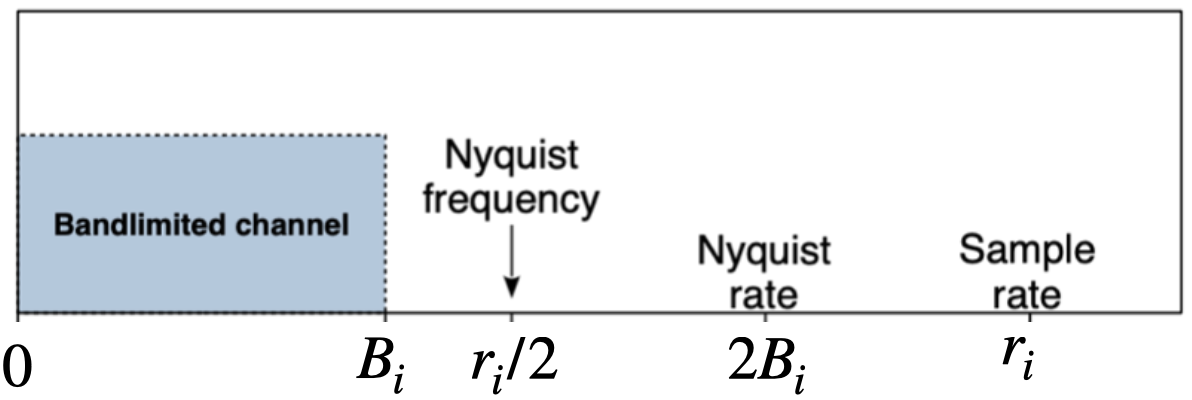
\includegraphics[width=0.7\linewidth]{img/ch4/nyquist.png}
\caption{Nyquist Limit.}
\label{f:nyquist}
\end{figure}


Therefore, to fit the stage $g_i$ to the sample $\{\gt{g}_i(x_{kl})\}$, we initialize its parameters to handle frequencies up to $\omega_i = \frac{r_i}{2}$. We do this by uniformly sampling the rows of the first matrix $W_{s_i}$ in the set $\Omega_i = \left[-\omega_i, \omega_i\right]^2$. For the S-Net model, we set $\omega = r_i$. For the L-Net and M-Net models, we constrain $\omega$ to the range $\frac{r_i}{32} \leq \omega \leq \frac{r_i}{8}$, depending on the depth of the network. This adjustment accounts for the fact that the composition of sinusoidal layers can generate significantly higher frequencies. Additionally, note that the first sinusoidal layer $S_i$ may reuse some frequencies initialized in earlier stages, since $\Omega_0 \subset \cdots \subset \Omega_{N-1}$.


\subsection{Loss Functional}

We aim to fit the MR-Net $f$ to the ground-truth signal $\gt{f}$ based on a sampled subset of $\gt{f}$. This process is essentially a multiscale regression, where: (i) the approximation must account for the multiresolution decomposition $\gt{f} = \gt{g}_0 + \cdots + \gt{g}_{N-1}$ of the ground-truth signal, and (ii) each MR-Net stage $g_i$ should fit to a sample of $\gt{g}_i$.

To accomplish these goals, we define a \textit{loss functional} $\mathcal{L}_i$ to train each stage $g_i$ of the MR-Net $f$. Suppose the signal $\gt{f}$ has been sampled and organized into a \textit{multi-stage stack} $\{x_j, y_j\}_i$, where $y_j = \gt{g}_i(x_j)$. The loss function $\mathcal{L}_i$ is then defined as minimizing the squared difference between the true values $y_j$ at the sample points $x_j$ and the predicted values $g_i(x_j)$ at the $i$th stage:

\begin{align}\label{e-loss}
    \mathcal{L}_i(\theta_i)=\frac{1}{K_i}\sum \norm{g_i(x_j)-y_j}^2.
\end{align}

where $\theta_i$ are the parameters of $g_i$, and $K_i$ is the size of the multi-stage stack $\{x_j, y_j\}_i$.

% When the multi-stage stack $\{x_j, y_j\}_i$ is constructed by filtering $\gt{f}$ using a Gaussian filter (Eq~\ref{e-gaussian-filter}), we should replace $\norm{g_i(x_j)-y_j}$ by $\norm{f_i(x_j)-y_j}$ in Eq~\ref{e-loss}, recall that $f_i$ is the $i$th level of detail of the MR-Net $f$, i.e. $f_i=g_0+\dots+g_{i}$.

If the multi-stage stack $\{x_j, y_j\}_i$ is constructed by filtering $\gt{f}$ using a Gaussian filter (Equation \ref{e-gaussian-filter}), we modify the loss function by replacing $\norm{g_i(x_j) - y_j}$ with $\norm{f_i(x_j) - y_j}$ in Equation \ref{e-loss}. Recall that $f_i$ represents the $i$th level of detail of the MR-Net, defined as $f_i = g_0 + \dots + g_i$. This ensures that the cumulative effect of all stages up to $g_i$ is considered during training.

% Consequently, a good loss function bridges the gap between the data and the functional model.
% The most common \textit{norms} for regression problems use the $L^1$ and $L^2$ norms.

% During training, the network can be over-fitted to the data. To avoid this, we explore regularization strategies such as defining convergence criteria for early stopping to fit the network to the data. In the future, we plan to enhance these strategies by adding \textit{regularization terms} based on network derivatives. 

\subsection{Scheduler}


The multiresolution training process is managed by a training scheduler, which organizes the training sequence and applies regularization strategies based on convergence criteria. In our experiments, we implement a scheduler to train each stage sequentially, from the lowest resolution to the highest. However, when the input multi-stage stack $\{x_j, y_j\}_i$ is structured as a Laplacian pyramid and $f$ is an L-Net, it becomes possible to train all stages in parallel by summing the loss functions $\mathcal{L}_i$ of the MR-stages.

We further employ a progressive learning strategy, where the weights of each stage are "frozen" after it has been trained. This ensures that details are added to the network incrementally, moving from coarse to fine resolution, which promotes stability in training. Additionally, we use an adaptive training scheme for optimizing each stage, which combines accuracy-based loss thresholds and convergence rate monitoring. This adaptive approach helps fine-tune the training process, improving computational efficiency for each stage.
% and prevents overfitting to finer details too early in the process.

In practice, several additional operations are performed throughout the training process. These may include saving model checkpoints, logging the current value of the loss function, and generating plots or visualizations of intermediate and final results. As such, the scheduler is also responsible for issuing notifications at key points during training, such as when training begins, when a data batch has completed, or when a specific stage starts or finishes. This ensures that the training process is monitored and recorded systematically. The complete training procedure is outlined in Algorithm \ref{alg:mr-training}.

\begin{algorithm}[hbt!]
\KwData{A multi-stage stack $\{x_j, y_j\}_i$ with $N$ levels.}
\KwResult{A MR-Net $f$ with $N$ stages $g_i$.}
    Initialize a MR-Net model with a single stage $g_0$\;
    Notify that network training will start\;
    \For{$stage\gets0$ \KwTo $N-1$}{
        \If{$stage\neq~0$}
        {
            Create a new stage $g_{stage}$ and add it to the model\;
            Freeze the parameters of the stage $g_{stage-1}$\;
        }
        Notify that stage training will start\;
        $\texttt{current\_traindata}~\!\!\gets~\!\!\texttt{multires\_stack}[stage]$\;
        \For{\normalfont $epoch\gets 0$ \KwTo \texttt{current\_limit\_of\_epochs}}{
            \For{\normalfont \textit{batch} in \texttt{current\_traindata}}{
                Train $g_{stage}$ using the loss $\mathcal{L}_{stage}$ (Eq~\ref{e-loss}) \;
                Notify that batch training has finished\;
            }
            Notify that epoch training has finished\;
            \If{\normalfont\texttt{convergence\_criteria\_reached()}}
                {\textbf{break}\;}
        }
        Notify that stage training has finished\;
    }
    Notify that network training has finished\;
    \caption{MR-Net training procedure.} 
    \label{alg:mr-training}
\end{algorithm}

\section{Multiresolution Inference}

A primary goal of a signal representation is to provide an accurate reconstruction of the underlying data. Ideally, the reconstruction method should be able to work with a continuous model of the signal, generating signal values at arbitrary points of its domain. Coordinate-based neural networks provide a compact and continuous representation of signals, and our MR-Net architecture extends this concept by offering continuity both in space and scale. Therefore, it can reconstruct the signal zooming in and out at varying levels of detail by adjusting the control layer coefficients through a parameter $t$ during inference, as described in Equations~\ref{e-mrnet} and \ref{e-control}.
% In that respect, coordinate-based neural networks features a compact model of the signal as a continuous function. Additionally, our MR-Net architecture gives a representation that is continuous both at space and scale. 
% Therefore, it can reconstruct the signal zooming in and out at any desired level of detail by specifying a value $t$ to adjust the control layer coefficients, during the inference, according to Equations \ref{e-mrnet} and \ref{e-control}.

These characteristics are particularly valuable in media applications, where controlling signal reconstruction is essential for rendering and adapting to different display resolutions. MR-Net's ability to filter frequency content in a controlled manner makes it ideal for handling \textbf{antialiasing}, a critical process that prevents visual artifacts during rendering.

The hierarchical structure of MR-Net, with its levels of detail, has important implications for both signal transmission and processing. For transmission, coarse versions of the signal can be sent quickly through a channel, with subsequent updates refining the level of detail for progressive rendering. For processing, the multiresolution approach facilitates data caching and the efficient use of memory structures of the GPU, enabling performance optimization across different stages of the rendering pipeline.

% \section{MR-Framework}


% % \vspace{0.2cm}
% % {\color{red}
% % In practice, we assume that the data is given as a regular sample (digital image) of size $2^{k}\times 2^k$
% % of the ground-truth signal~$\gt{f}$.
% % We abuse the notation by denoting this digital image by~$\gt{f}$.
% % To train the MR-Net stages~$\{g_i\}$, we use the (discrete) \textit{Gaussian} and \textit{Laplacian} pyramids of $\gt{f}$, both with $N<k$ levels.
% % Precisely, the Gaussian pyramid $\{\gt{f}_i\}$ is defined recursively by convolving the \textit{level of detail} $\gt{f}_i$ with a Gaussian kernel $K$ and downsampling the result by a factor 2:
% % \begin{align*}
% %     \gt{f}_i(k,l)&=\left(K*\gt{f}_{i+1}\right)(2k,2l)\,\, \text{with} \,\, k,l\in \left\{1,\ldots, 2^{k-N+1+i}\right\},\\
% %     \gt{f}_{N-1}&=\gt{f}.
% % \end{align*}
% % $\gt{f}_i(k,l)$ denotes the digital image $\gt{f}_i$ evaluated at the pixel $(k,l)$.
% % Similarly, the Laplacian pyramid $\{\gt{g}_i\}$ is defined using
% % \begin{align*}
% %     \gt{g}_i(k,l)&=\left(\gt{f}_{i}-K*\gt{f}_{i}\right)(2k,2l)\,\, \text{with} \,\, k,l\in \left\{1,\ldots, 2^{k-N+1+i}\right\}\\ \gt{g}_0(k,l)&=\left(K*\gt{f}_{1}\right)(2k,2l).
% % \end{align*}
% % Since $2^{k-N+1+i}$ is the height and width of $\gt{g}_i$, it cannot contain frequencies higher than $\omega_i=2^{k-N+i}$. 
% % Thus we propose to initialize the frequencies of the $N$ stages $\{g_i\}$ of the MR-Net $f$ following a dyadic sequence of frequency bands 
% % \begin{align}
% % \omega_{N-1}, \omega_{N-2}, \ldots, \omega_{0}.
% % \end{align}
% % Which is equivalent to $\omega_{N-1}, \frac{\omega_{N-1}}{2}, \ldots, \frac{\omega_{N-1}}{2^{N-1}}$ with $\omega_{N-1}= 2^{k-1}$.
% % These are the bandlimits used to define the sets $\Omega_i=\left[-\omega_i, \omega_i\right]^2$ to initialize the frequencies of the first layer of each stage $g_i$.
% % (see Fig~\ref{f:freq-bands}).

% % \begin{figure}[!h]
% % \centering
% % \includegraphics[width=0.98\linewidth]{figs/freq-bands.png}
% % \caption{Frequency Bands}
% % \label{f:freq-bands}
% % \end{figure}

% % }


% % \section{MR-Net in Detail}
% % \label{sec:mrnet_detail}

% This section presents the MR-Net framework in detail by conceptually dividing it in four main components: \emph{MR-Structure}, \emph{MR-Stages}, \emph{MR-Training}, and \emph{MR-Inference} (see Fig~\ref{f:components}).

% % Let $\gt{f}:\mathcal{D}\to \mathcal{C}$ be the ground-truth signal (\textit{input data}), and $f\!:\!\mathcal{D}\!\times\! [0,N]\!\to\! \mathcal{C}$ be a MR-Net with $N$ stages $\{g_i\}$ to fit $\gt{f}$~in multiresolution.
% % We use this setting to present the framework.

% \subsection{MR-Structure}\label{sec:mr_struct}

% The MR-Structure is a data structure that encapsulates the input data $\gt{f}$. It includes $\gt{f}$ and metadata about its \textit{sampling mode}, \textit{filtering type}, and the \textit{multi-stage stack} (see Fig~\ref{f:structure}).
% \begin{figure}[!h]
% \centering
% 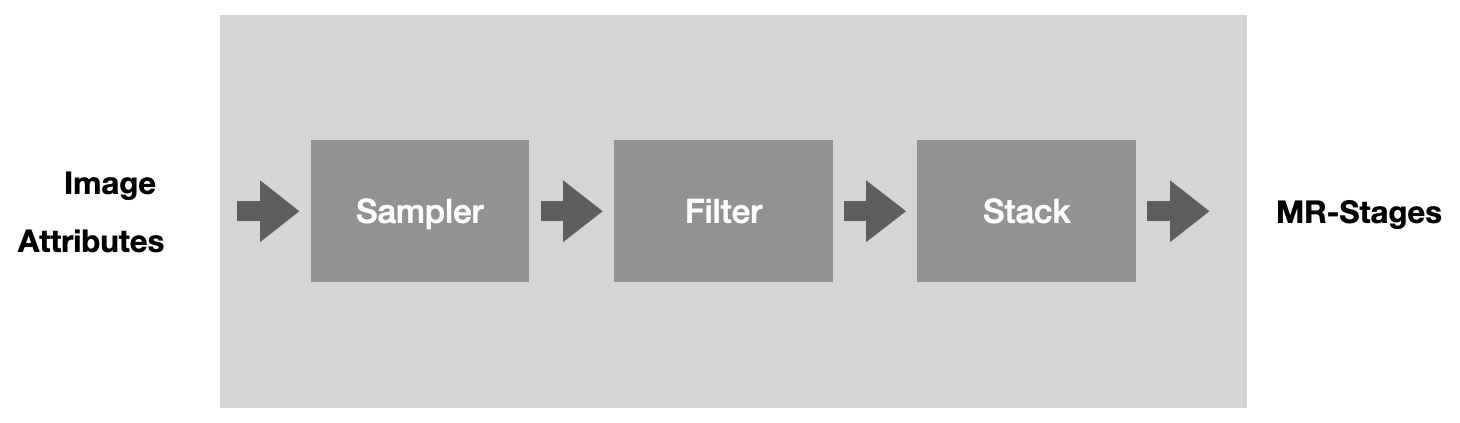
\includegraphics[width=0.89\linewidth]{img/ch4/mr-structure.png}
% \caption{MR-Structure.}
% \label{f:structure}
% \end{figure}



% \subsection{Logger}

% The training of the MR-Net $f$ is monitored by a logging module that helps to visualize the learning progress. During training, the logger receives messages when the network training starts and ends, when a stage training starts and ends, when a epoch training ends, and when a batch training ends. 

% This architecture allows the logger to be customized to accommodate different MR-Net configurations and different actions for visualizing the training progress. For instance, it is possible to write a logger to save partial results to the disk, display~them in a development environment, or send them to a cloud based~service.
